\documentclass[../main/main.tex]{subfiles}
\begin{document}

\chapter{Cr\'eation d'un \'echantillon complet}\label{ch:sample}

\epigraph{Citation}{Autaire}
Afin d'améliorer l'état de l'art dans le domaine de la cosmologie
observationnelle à l'aide de SNe~Ia et en vue de tester l'évolution de leurs
propriétés avec le reshift, la première étape de ce projet a été de choisir
l'échantillon d'étude.

% \dominitoc
% \tableofcontents
\vfill
\minitoc
\vfill
\newpage

\section{Notion de complétude}\label{sec:compl}

% Malmquist bias :~\cite{perrett2010}

Cette thèse repose sur l'étude statistique des propriétés des SNe~Ia, et  donc
en premier lieu sur l'échantillon de données sur lesquelles développer notre
raisonnement. Pour qu'il soit intéressant il doit être suffisamment grand, mais
également représentatif de la population des SNe~Ia, c'est-à-dire au plus proche
d'être un tirage aléatoire de tout ce qu'il peut exister comme SNe~Ia dans la
nature. On parle alors d'échantillon complet. Ce concept est donc largement
dépendant de la manière dont les données sont relevées.

\subsection{Stratégies d'observations}\label{ssec:startobs}

Les supernovae sont des phénomènes transitoires, c'est-à-dire des objets dont le
flux lumineux varie dans le temps, mais elles sont également brèves et rares~:
elles durent typiquement quelques semaines et surviennent environ une fois par
siècle et par galaxie. Leur observation requiert donc des stratégies
particulières. Pour déterminer leurs courbes de lumière (\ref{ssec:lc}) il est
nécessaire d'avoir un champ de mesure suffisamment profond pour ne pas se
contenter que de leur luminosité au maximum. Différentes approches peuvent
entrer en jeu~: les recherches ciblées et les recherches non ciblées.

\paragraph*{Les recherches ciblées} consistent à se focaliser sur des amas de
galaxies connus en vue d'augmenter la probabilité d'observer des supernovae~; il
paraît en effet évident que plus la concentration en étoiles est forte, plus on
s'attend à avoir une haute probabilité que certaines d'entre elles entament leur
fin de vie et leur explosion en supernova. Cependant, une telle pratique
implique une sélection des environnements des SNe et donc un biais sur la nature
des données recueillies~; dans le cas des amas de galaxies, l'environnement
favorisé sera celui contenant des progéniteurs vieux, dans des galaxies massives
avec peu de formation stellaire. Afin d'étudier la potentielle évolution de la
population des SNe, il faut réduire au maximum ces biais et favoriser la récolte
d'un échantillon représentatif de toute la zoologie des SNe~Ia.

\paragraph*{Les recherches non-ciblées} utilisent de grands champ de caméra pour
sonder de larges portions du ciel. Originellement
\citep[SCP,][]{perlmutter1999}, leur procédé était d'effectuer une
détection photométrique avant d'opérer une identification spectroscopique,
confirmant leur caractère de SN~Ia ou non, pour finalement décider de programmer
ou non un suivi photométrique permettant l'établissement de leur courbe de
lumière. Une telle pratique limite les biais mais donne des courbes de lumières
pauvres en points de mesure avant le maximum de luminosité, impactant
l'ajustement des courbes. Ces méthodes ont évolué pour devenir des recherches
\textit{glissantes}~\citep{astier2006}. Elles consistent à balayer régulièrement
le ciel en observant un même champ dans un même filtre de manière répétée tous
les quelques jours, afin d'à la fois détecter et extraire les courbes de
lumières des SNe~Ia, même si leur identification est effectuée après leur
maximum de luminosité.

\subsection{Biais de Malmquist et solution}\label{ssec:malm}

De tels sondages ne sont cependant pas exempts d'effets de sélection. En effet,
même une recherche glissante s'effectue avec un appareil de mesure ayant une
capacité limitée à détecter une source lumineuse~: les objets de magnitude
apparente plus élevée (luminosité plus faible) que ce seuil de détection ne
seront pas inclus. Or, comme chaque astre voit sa luminosité décroître avec le
carré de la distance qui le sépare de l'observation (\ref{ssec:dl}), cette
limite implique que les astres de magnitude absolue plus élevée seront relevés à
de plus grandes distances que les autres, laissant croire qu'à partir d'une
certaine distance les objets sont intrinsèquement plus lumineux.

Dans le cadre des SNe~Ia dont on suppose la magnitude absolue similaire, on
pourrait en première approche négliger cet effet. Cependant, comme exposé en
Section~\ref{ssec:corr}, il a été déterminé que la magnitude absolue des
supernovae de type Ia est corrélée avec leur \textit{stretch} et leur couleur de
telle sorte que les plus faibles soient celles de petit stretch et de couleur
rouge. Ainsi, proche du seuil de détection, les SNe~Ia ne sont pas sélectionnées
de manière homogène, et l'échantillon recueilli sera une sous-population
laissant penser qu'avec la distance, les SNe~Ia ont en moyenne un plus haut
stretch et sont de couleur bleue. De tels sondages sont dits à magnitude
limitée.

Le cadre de notre étude nécessite un échantillon qu'on appelle
«~volume-limité~», pour lequel on suppose que la population résulte bien d'un
tirage aléatoire de ce qui existe dans la nature. Les sondages modernes reposant
sur des recherches glissantes, il nous a donc fallu les réduire pour les
utiliser.

\section{Présentation des sondages}\label{sec:surveys}
On présente dans cette section les différents sondages utilisés dans notre
étude, principalement non-ciblés. La Table~\ref{tab:sondcomp} présente la
comparaison des caractéristiques des sondages.

\subsection{The Nearby Supernova factory}\label{ssec:snf}
\subsubsection{Introduction}\label{sssec:snfintro}

La collaboration \textit{The Nearby Supernova factory}
\citep[SNfactory,][]{aldering2002} est créée peu de temps après la découverte de
l'expansion accélérée de l'Univers~\citep{riess1998, perlmutter1999} avec pour
but un suivi spectro-photométrique d'une précision d'environ 1\% de SNe~Ia
proches. L'objectif est de peupler la partie basse du diagramme de
\textsc{Hubble} ($0,03 < z < 0,08$), qui ne contenait alors qu'une vingtaine de
SNe~Ia \citep{hamuy1996}, permettant une meilleure détermination de la constante
de \textsc{Hubble} $H_0{}^2$. La faible distance du sondage permet d'éviter
d'appliquer des corrections photométriques dues au redshift
(corrections $K$, voir Section \textbf{?}). La mission tente également d'étudier
précisément les propriétés des SNe~Ia grâce au traceur LsSFR (Section
\textbf{?}) afin de mieux comprendre leur diversité, mettre en évidence
différentes populations de supernovae et améliorer leur standardisation grâce à
une meilleure compréhension de leurs variabilités et ainsi réduire les erreurs
systématiques dans les mesures de paramètres cosmologiques.

\subsubsection{Détection des supernovae}\label{sssec:snfdetec}

Le programme a été sujet à plusieurs évolutions au cours de son fonctionnement,
notamment pour la découverte de nouveaux candidats. Ce sont d'autres télescopes
qui alertent la communauté. En premier lieu, jusqu'à fin 2008, le télescope de
\SI{1,2}{m} du mont Palomar en Californie~\citep{rabinowitz2003} scannait
\SI{500}{deg^2} du ciel chaque soir avec la caméra QUEST de 112 capteurs CCD. À
partir de 2010, les canditats de SNe proviennent d'une coopération avec
\textit{Palomar Transient Factory}~\citep[PTF,][]{law2009} et de données
publiques. La caméra QUEST fut ensuite déplacée à La Silla au Chili
\citep[LSQ,][]{hadjiyska2012} pour reprendre, mi-2012, l'activité de recherche
de SNe pour SNfactory. Les candidats potentiels sont à chaque fois programmés
pour observation spectroscopique afin de les identifier en tant que SNe~Ia et
décider de leur suivi selon des critères de qualité (nombre de points de mesure,
proche et avant du maximum, non-contamination pas la luminosité de la Lune
notamment). Les transmissions des filtres $B$ et $V$ de La Silla sont tracées
Figure~\ref{fig:snfbands}.

\begin{figure}[ht]
    \centering
    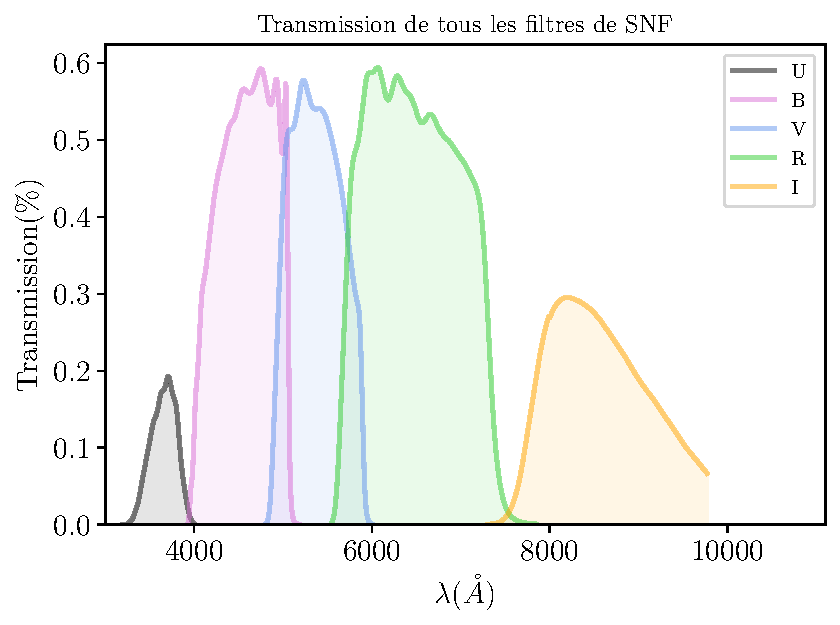
\includegraphics[width=.8\linewidth]{bands_SNF.pdf}
    \captionsetup{justification=centering}
    \caption{Transmissions des filtres de La Silla utilisés par SNF.}
    \label{fig:snfbands}
\end{figure}

\subsubsection{Suivi spectro-photométrique}\label{sssec:snfspectro}

Le typage spectroscopique, quand il n'a pas déjà été réalisé par d'autres
collaboration ayant donné l'alerte, est assuré par le \textit{SuperNovae
Integral Field Spectrograph}~\citep[SNIFS,][]{lantz2004} du télescope de
l'Université d'Hawaii de \SI{2,2}{m} au sommet du Mauna Kea, mis en service en
2004. Il s'avère plus efficace qu'un typage photométrique qui nécessite
plusieurs observations dans différents filtres de couleur, bien que ces
dernières soient plus simple à mettre en place.

Ce spectrographe dit «~à champ intégral~» récolte des «~cubes~», des données en
3 dimensions, deux spatiales représentant un point dans le ciel plus une
dimension de longueur d'onde~; chaque point de ce relevé se nomme
\textit{spaxel}, pour «~spatial picture element~», et ensemble forment une
grille de 15 $\times$ 15 pour un champ de vue total de \ang{;;6,4} $\times$
\ang{;;6,4} dans deux longueurs d'ondes~: une voie bleue ($B$) de 3200 à
\SI{5200}{\angstrom} et une voie rouge ($R$) de 5100 à \SI{10000}{\angstrom}.

En plus de cette voie, SNIFS possède une voie photométrique utilisant 5 filtres
$ugriz$ pour suivre l'absorption atmosphérique, et une voie de guidage avec un
filtre $V$ pour aider le télescope à la focalisation. Le champ de ces caméras
est de \ang{;4,5;} $\times$ \ang{;9;}.

\subsubsection{Taux de formation stellaire spécifique
spectroscopique}\label{sssec:snflssfr}

La spécificité de SNIFS est de permettre des mesures spectroscopiques de
l'environnement immédiat des SNe, développée dans~\cite{rigault2013} et résumée
dans~\cite{rigault2020}. Ce procédé commence par modéliser le spectre du ciel
qui est soustrait aux cubes avant d'extraire le spectre de l'environnement dans
un rayon de \SI{1}{kpc} projeté autour de la position des SNe~Ia. Ces données
permettent de détecter l'émission de raies H$\a$, l'un des indicateurs
traditionnellement les plus utilisés pour mesurer le taux de formation stellaire
(\textit{stellar formation rate}, SFR~; cf.~\cite{kennicutt1998}), en
l'occurrence dans l'environnement local (à moins de \SI{1}{kpc}). Il repose sur
le fait que les étoiles massives ($\gtrsim \SI{20}{\Msun}$) génèrent des photons
ultra-violets (donc à haute énergie) capables d'ioniser les gaz d'hydrogène de
leur environnement \citep{calzetti2012} en grande quantité. Ces atomes excités
vont ensuite se recombiner, produisant diverses raies d'émission dont certaines
dans la série de \textsc{Balmer}. C'est ce principe qui fournit les raies H$\a$,
dont la longueur d'onde dans le vide est $\lambda_{\mathrm{H}\a} =
\SI{656.5}{nm}$. L'étude de cette raie permet l'estimation de la formation
stellaire du fait que les étoiles massives ont une courte durée de vie, à
l'échelle de millions d'années, et que leur capacité à générer de tels photons
décroît très rapidement~: le flux généré décroît de deux ordres de grandeurs
en approximativement \SI{10}{Mans}. La présence d'hydrogène ionisé est donc un
indicateur direct de la présence de «~jeunes~» étoiles, c'est-à-dire de moins de
\SI{100}{Mans}, et de taux de formation stellaire \textit{via} la
correspondance~:
\begin{equation}
    \mathrm{SFR}(\mathrm{H}\alpha) = 5,45\times 10^{-42}L(\mathrm{H}\a)
\end{equation}
avec $L(\mathrm{H}\a)$ la luminosité des raies d'émission.

\NN{Description principe}

\subsubsection{Description des données conservées}\label{sssec:snfdata}

De 2004 à 2013, SNfactory a classifé 1364 objets dont plus de 1000 supernovae,
observé 645 SNe~Ia au moins une fois et en a suivi plus de 271 SNe~Ia, avec au
moins 5 points de mesure~\citep{copin2013}.

Sur celles-ci, 198 ont des mesures satisfaisant les contraintes nécessaires à
l'établissement de leur courbe de lumière et sont associées à une galaxie hôte
permettant de déterminer leur redshift~; pour efficacement déterminer les
propriétés locales de leur environnement, seules les SNe entre $z = 0,02$ et $z
= 0,08$ sont conservées, amenant l'échantillon à 160 objets.

Les données pour lesquelles les images des galaxies hôtes dans les bandes
photométriques $g$ et $i$ sont contaminées par la luminosité des SNe sont
également rejetées~; ces bandes s'avèrent en effet nécessaires à la
détermination de la masse stellaire de la galaxie. Cette coupe réduit
l'échantillon à 147 objets.

Les SNe considérées comme trop «~anormales~» sont exclues car supposées non
représentatives de la population générale que l'on souhaite étudier. Elles sont
au nombre de 6.

Finalement, parmi ces 141, ne sont conservées que celles provenant directement
des collaborations internes \NN{ou uniquement celles SNIFSées ?}, c'est-à-dire
celles de SNf, PTF et LSQ. L'échantillon final est alors de 114 données.  
L'ensemble de ces critères de sélection est résumé Table~\ref{tab:snfcuts}.

Grâce au suivi spectroscopique de tous les candidats à $r \lesssim
\SI{19,5}{mag}$ et ces limitations en redshift, ces données sont considérées
comme étant limitées en volume, c'est-à-dire un tirage aléatoire des populations
sous-jacentes de SNe~Ia.

\begin{table}[]
    \centering
    \caption{Critères de sélection des SNe~Ia suivies par SNfactory.}
    \label{tab:snfcuts}
    \begin{tabular}{lc}
        \toprule
        Critères de sélection           & Nb de SNe~Ia \\
        \midrule
        Suivies                         & 271 \\
        Courbe de lumière + hôte        & 198 \\
        $0,02 < z < 0,08$               & 160 \\
        Hôte $g$ et $i$ non contaminées & 147 \\
        SNe~Ia «~normales~»             & 141 \\
        SNf LSQ ou PTF seulement        & 114 \\
        \bottomrule
    \end{tabular}
\end{table}

\begin{figure}[ht]
    \centering
    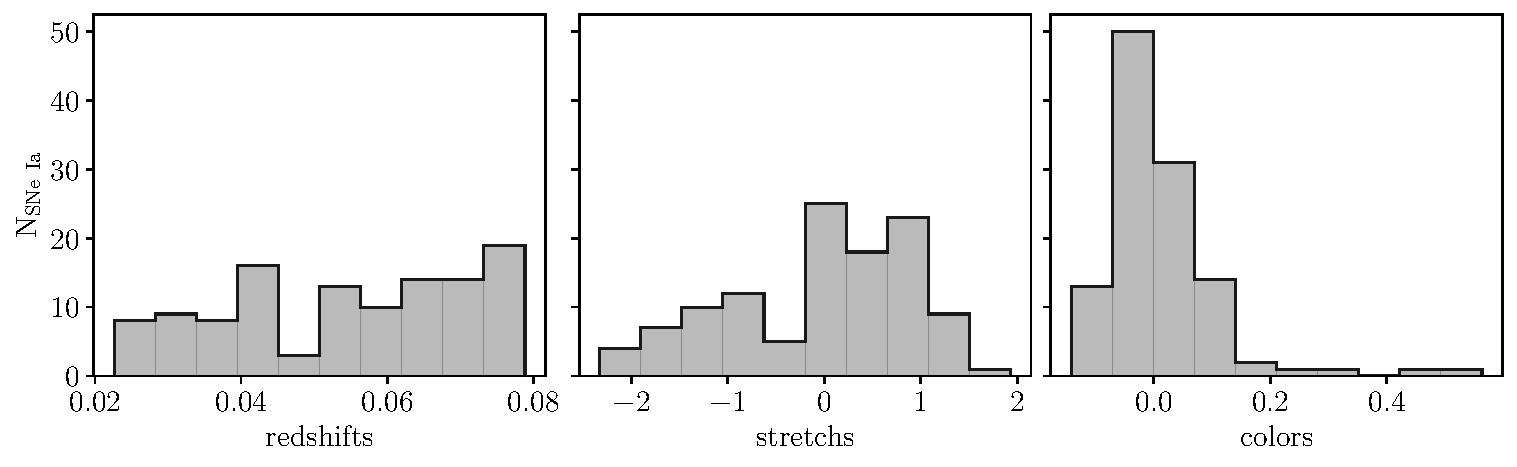
\includegraphics[width=\linewidth]{hist_SNF_zxc.pdf}
    \captionsetup{justification=centering}
    \caption{Distributions des paramètres de redshift (à gauche), de stretch (au
    milieu) et de couleur (à droite) pour les 114 données de SNfactory.}
    \label{fig:snfhist}
\end{figure}

\subsection{Sloan Digital Sky Survey}\label{ssec:sdss}
\subsubsection{Introduction}\label{sssec:sdssintro}

Le \textit{Sloan Digital Sky Survey}~\citep[SDSS,][]{frieman2008, sako2008,
sako2018} est un sondage astronomique majeur qui a débuté en 2000 et est encore
actif aujourd'hui. Le programme se divise en cinq phases d'observation de
différents objets astrophysiques, de simples étoiles aux grandes structures de
l'Univers. La partie supernova du sondage est une des trois composantes de la
seconde phase et s'étend de 2005 à 2008~; ce sera la seule que nous détaillerons
ici. Son objectif principal est de répondre au manque de données astrophysiques
à redshifts intermédiaires par rapport aux sondages de l'époque~: l'intervalle
de redshifts sondés est entre $0,05 \lesssim z \lesssim 0,45$, partie encore peu
peuplée en 2005. À cela s'ajoute la volonté de réduire les limitations
systématiques des autres programmes afin d'améliorer les contraintes sur les
propriétés de l'énergie sombre, par l'utilisation de sa combinaison unique de
couverture céleste, précision photométrique et grande sensibilité. Ceci est
rendu possible grâce à la première phase du sondage qui a apporté un large base
de données d'images de références, de catalogue d'objets et de calibration
photométrique.

\subsubsection{Détection des supernovae}\label{sssec:sdssdetec}

La stratégie d'observation de SDSS se concentre sur \SI{300}{deg^2} du ciel
faiblement affectée par l'extinction galactique, nommée Bande 82, en y répétant
l'acquisition. Elle est réalisé grâce au télescope optique dédié de \SI{2,5}{m}
\citep{gunn2006} à Apache Point au Nouveau Mexique, couplé à une caméra CCD
\citep{gunn1998} à 5 filtres optiques~\citep[$ugriz$,][]{fukugita1996} qui
tournent avec une cadence relativement haute, environ une acquisition toutes les
4 à 5 nuits. Les transmissions de ces filtres sont tracées
Figure~\ref{fig:sdssbands}. Le procédé d'acquisition est similaire à celui de
SNf, étant tous les deux des sondages à recherche glissante~: différentes images
du ciel sont comparées pour détecter les phénomènes transitoires et créer des
courbes de lumière. Cette stratégie a permis à SDSS de détecter la majeure
partie de ses SNe bien avant leur maximum d'émission (pour $z \lesssim 0,3$)
avec des courbes bien échantillonnées en plusieurs bandes photométriques (cf.
Figure~\ref{fig:sdsslc}).

\begin{figure}[ht]
    \centering
    \begin{subfigure}[]{.49\linewidth}
        \centering
        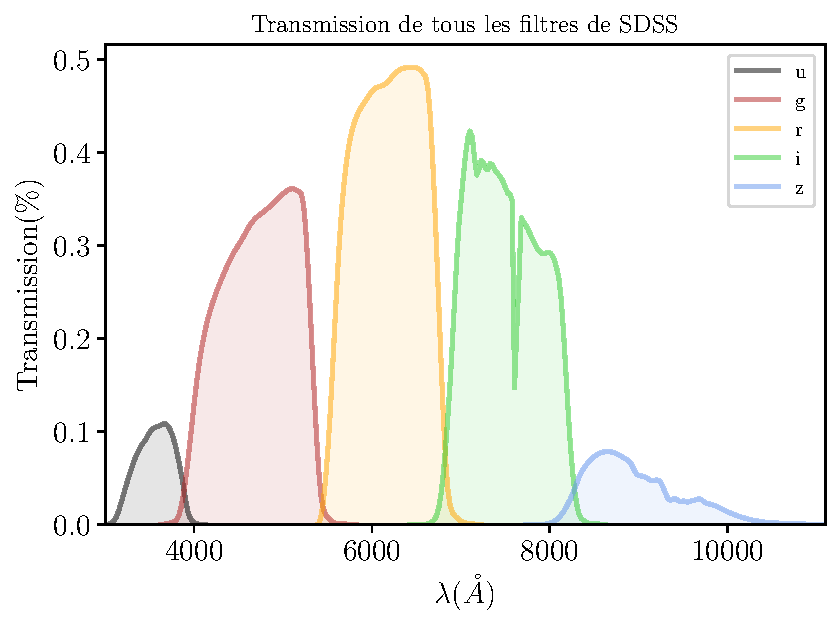
\includegraphics[width=\linewidth]{bands_SDSS.pdf}
        \captionsetup{justification=centering}
        \caption{Transmissions des filtres utilisés par le sondage SDSS.}
        \label{fig:sdssbands}
    \end{subfigure}
    \begin{subfigure}[]{.49\linewidth}
        \centering
        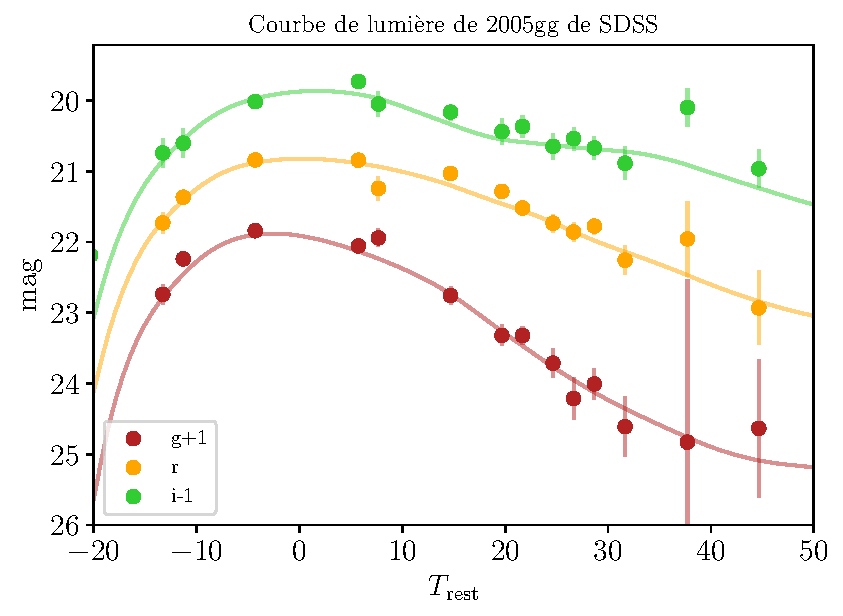
\includegraphics[width=\linewidth]{lc_2005gg.pdf}
        \captionsetup{justification=centering}
        \caption{Courbe de lumière en bandes $gri$ de la SN~Ia
            confirmée 2005gg, à $z = 0,230$.}
        \label{fig:sdsslc}
    \end{subfigure}
    \caption{Caractéristiques du sondage SDSS.}
\end{figure}

% \begin{figure}[ht]
%     \centering
%     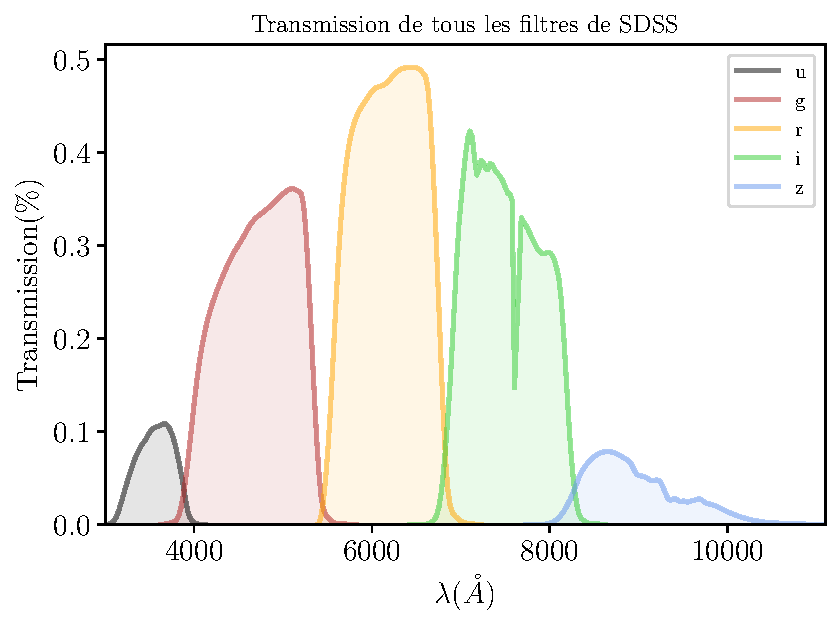
\includegraphics[width=.8\linewidth]{bands_SDSS.pdf}
%     \captionsetup{justification=centering}
%     \caption{Transmissions des filtres de SDSS.}
%     \label{fig:sdssbands}
% \end{figure}
% 
% \begin{figure}[ht]
%     \centering
%     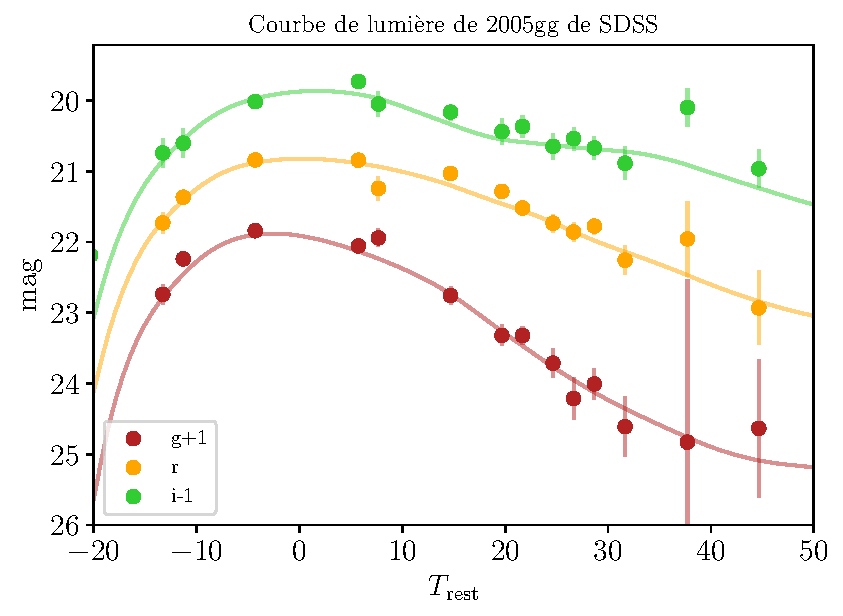
\includegraphics[width=.8\linewidth]{lc_2005gg.pdf}
%     \captionsetup{justification=centering}
%     \caption{Courbe de lumière en bandes $gri$ de la supernova SN 2005gg, une
%     SN Ia confirmée à $z = 0,230$. Le temps est compté en jours relativement au
% pic d'émission en bande $g$. Figure reproduite de~\cite{frieman2008}.}
%     \label{fig:sdsslc}
% \end{figure}

Pour discriminer entre bruit de fond et réelle variation astronomique, une
inspection visuelle par un humain était systématiquement nécessaire jusqu'en
2006, \textit{via} une interface web comportant les images dans les filtres
$gri$ et d'autres informations pertinentes. Des 5 filtres utilisés, ce sont donc
ces trois-là qui forment les meilleures mesures. Après cette date, la détection
est en partie laissée au logiciel \textit{autoscanner}. Sur les trois saisons
d'observation, ce sont 10258 nouveaux objets transitoires qui ont été
découverts.

\subsubsection{Suivi spectro-photométrique}\label{sssec:sdssspectro}

Le typage de SDSS utilise de nombreux différents télescopes~: le HET de
\SI{9,2}{m}~\citep{hill1998}, le
ARC\footnote{\href{http://www.apo.nmsu.edu/arc35m/Instruments/DIS/\#B}
{http://www.apo.nmsu.edu/arc35m/Instruments/DIS/\#B}} de \SI{3,5}{m}, Subaru de
\SI{8,2}{m}~\citep{kashikawa2000}, le
WHT\footnote{\href{http://www.ing.iac.es/PR/wht_info/whtisis.html}
{http://www.ing.iac.es/PR/wht\_info/whtisis.html}} de \SI{4,2}{m}, le
MDM\footnote{\href{http://www.astronomy.ohio-state.edu/MDM/CCDS/}
{http://www.astronomy.ohio-state.edu/MDM/CCDS/}} de \SI{2,4}{m}, le Keck de
\SI{10}{m}~\citep{oke1995}, le
TNG\footnote{\href{http://www.tng.iac.es/instruments/lrs/}
{http://www.tng.iac.es/instruments/lrs/}} de \SI{3,5}{m}, le NTT de \SI{3,6}{m}
\citep{dekker1986}, le
NOT\footnote{\href{http://www.not.iac.es/instruments/alfosc/}
{http://www.not.iac.es/instruments/alfosc/}} de \SI{2,5}{m}, les télescopes de
\textit{Magellan}\footnote{\href{http://www.lco.cl/magellan-telescopes/}
{http://www.lco.cl/magellan-telescopes/}} de \SI{6,5}{m} et le SALT de
\SI{11}{m}~\citep{burgh2003}~; plusieurs de ces télescopes pouvaient être prévus
pour observation la même nuit, rendant au total le temps alloué à la
spectroscopie supérieur au temps alloué à l'acquisition optique, permettant
l'acquisition de tous les candidats à $z \lesssim 0,15$.

Cependant, le nombre de candidat par nuit excède largement les capacités de
suivi spectroscopique, obligeant les opérateurs à faire une sélection des cibles
à analyser. Ainsi, un typage photométrique a également été réalisé en comparant
les courbes de lumière dans les bandes $gri$ avec des librairies de différents
modèles pour en estimer les paramètres (redshift, date du maximum de flux,
magnitude apparente, contamination galactique…) et permettre de prioriser les
cibles à suivre spectroscopiquement. Notamment, les SNe~Ia les plus prioritaires
sont celles qui sont bien séparées du centre galactique ($\gtrsim \ang{;;1}$),
avec un contraste de luminosité SN/galaxie raisonnable (critère visuel), et dont
la galaxie hôte est relativement rouge. Le sondage requiert généralement deux
détections avant le suivi spectroscopique, mais par manque de candidats à bas
redshift ce critère a pu être réduit contrairement aux données à $z \gtrsim 0,2$
où les candidats ne manquent pas. L'algorithme choisi par SDSS se rapproche
fortement de celui du sondage SNLS, cf Section~\ref{ssec:snls}.

En combinant les trois saisons d'observation, la phase II de SDSS a
spectroscopiquement confirmé 499 SNe~Ia~\citep{sako2018}.

\subsubsection{Données conservées}\label{sssec:sdssdata}

Après l'acquisition des données, une sélection supplémentaire s'applique pour ne
retenir que les données dites « cosmologiques », c'est-à-dire qui correspondent
aux exigences de qualité pour être insérées dans le diagramme de
\textsc{Hubble}. Pour SDSS, en appelant $T_{\rm rest}$ le temps en jours par
rapport au maximum d'émission en bande $B$, les critères sur les courbes de
lumière avancés dans~\cite{kessler2009b} sont les suivants~:

\begin{enumerate}
    \item Au moins 1 mesure avant $T_{\rm rest} < \SI{0}{jour}$~;
    \item Au moins 1 mesure après $T_{\rm rest} > \SI{10}{jours}$~;
    \item Au moins 5 mesures entre $-15 < T_{\rm rest} < \SI{60}{jours}$~;
    \item Au moins 1 mesure avec un rapport signal sur bruit > 5 en bande $g$,
        $r$ et $i$~;
    \item $\mathcal{P}_{\rm fit} > 0,001$, où $\mathcal{P}_{\rm fit}$ est la
        probabilité d'optimisation par degré de liberté donné par le programme
        \texttt{MLCS2K2}, similaire à \texttt{SALT2.4} (cf.
        Section~\ref{ssec:salt}).
\end{enumerate}
Dans l'analyse finale de~\cite{scolnic2018}, les données photométriques qui sont
considérées aberrantes ($>4\s$) sont retirées. Le nombre total de données
conservées est alors de 335. La Figure~\ref{fig:sdsshist} en présente les
histogrammes en redshift, stretch et couleur.

\begin{figure}[ht]
    \centering
    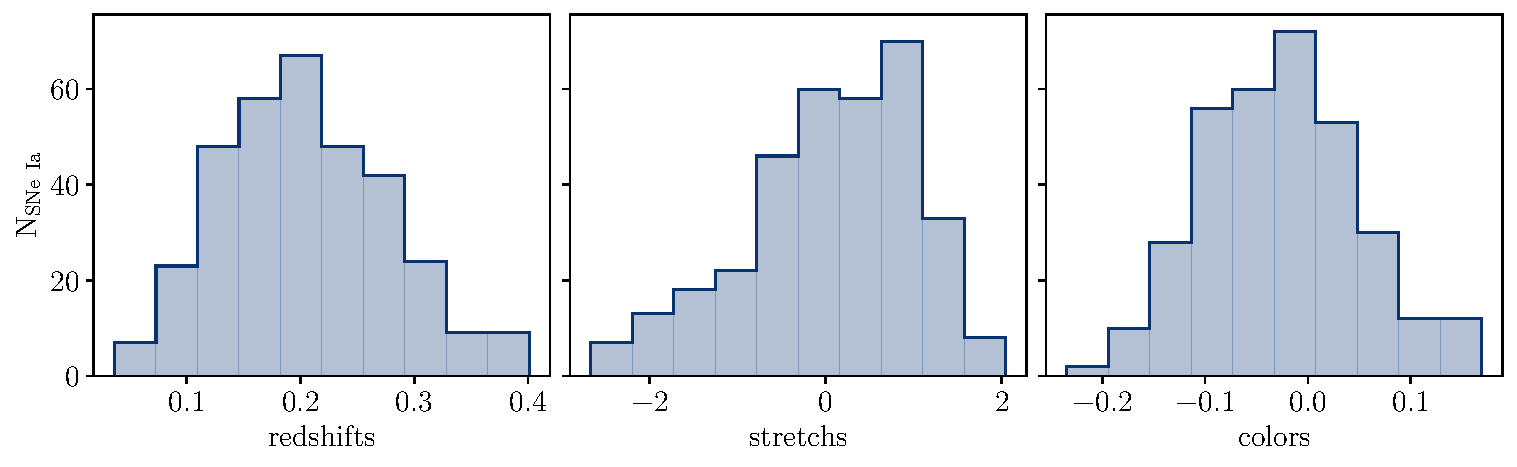
\includegraphics[width=\linewidth]{hist_SDSS_zxc.pdf}
    \captionsetup{justification=centering}
    \caption{Distributions des paramètres de redshift (à gauche), de stretch (au
    milieu) et de couleur (à droite) pour les 335 données de SDSS.}
    \label{fig:sdsshist}
\end{figure}

\subsection{Panoramic Survey Telescope and Rapid Response
System}\label{ssec:ps1}

\subsubsection{Introduction}\label{sssec:ps1intro}

Le \textit{Panoramic Survey Telescope and Rapid Response System}
\citep[Pan-STARRS,][]{chambers2016, scolnic2018} est un site d'imagerie et de
traitement de données astronomiques à grand champ, dont le premier télescope,
PS1 (se confondant par la suite avec le nom du sondage) est situé au sommet du
mont Haleakala sur l'île Maui de la chaîne d'îles hawaïenne. Son relevé a
commencé en 2009 pour se terminer en 2014. Son intervalle de redshifts sondés
s'étant de $0,02 < z < 0,65$, et ses objectifs scientifiques sont nombreux. Cela
inclut la photométrie de précision d'étoiles dans la Voie Lactée, le sondage du
système solaire avec recherche d'astres dangereux dans les environs de la Terre,
l'étude des phénomènes transitoires et la volonté de poser de nouvelles
contraintes sur l'énergie et la matière sombres. Ces deux derniers objectifs
sont ceux qui nous importent. 

\subsubsection{Détection des supernovae}\label{sssec:ps1detec}

Les relevés de PS1 sont réalisés grâce au sous-programme \textit{Medium Deep
Survey} (MDS) se concentrant sur 10 champs déjà bien étudiés de \SI{7}{deg^2}
chacun, pour une surface totale de \SI{70}{deg^2} et comptabilisant 25\% du
temps de PS1. Sa cadence est de 7 jours par filtre sur une période de 6 à
\SI{8}{mois} avec une profondeur de champ en bande $g$ de \SI{23,1}{mag}. Son
télescope~\citep{hodapp2004} est composé d'un miroir primaire de \SI{1,8}{m} et
d'un secondaire de \SI{0,9}{m}, couplés à la \textit{Gigapixel Camera \#1}
\citep[GPC1,][]{kaiser2010, tonry2006} observant une zone du ciel de \ang{3,3;;}
de diamètre. Les observations s'effectuent par l'utilisation combinées de 5
filtres $grizy_{\rm P1}$. Ils sont globalement similaires à ceux de SDSS (voir
Section~\ref{ssec:sdss}) à l'exception de la bande $g_{\rm P1}$ qui est
\SI{20}{nm} plus étendu du côté rouge du spectre et la bande $z_{\rm P1}$ qui a
une coupe plus nette à \SI{922}{nm}. Les transmissions des filtres sont tracées
Figure~\ref{fig:ps1bands}, et un exemple de courbe de lumière est présenté
Figure~\ref{fig:lc_550041}.

\begin{figure}[ht]
    \centering
    \begin{subfigure}[]{.49\linewidth}
        \centering
        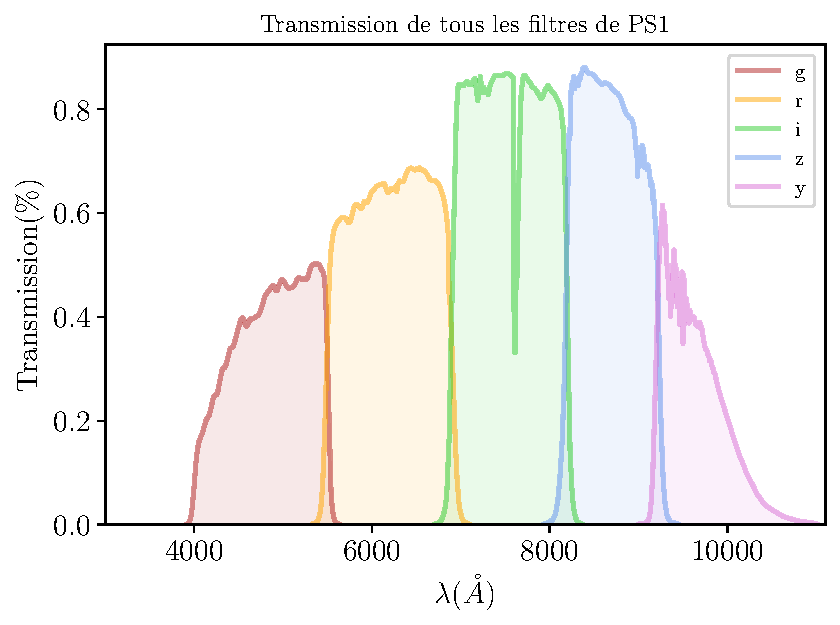
\includegraphics[width=\linewidth]{bands_PS1.pdf}
        \captionsetup{justification=centering}
        \caption{Transmissions des filtres $grizy$ de la caméra utilisée par
        PS1.}
        \label{fig:ps1bands}
    \end{subfigure}
    \begin{subfigure}[]{.49\linewidth}
        \centering
        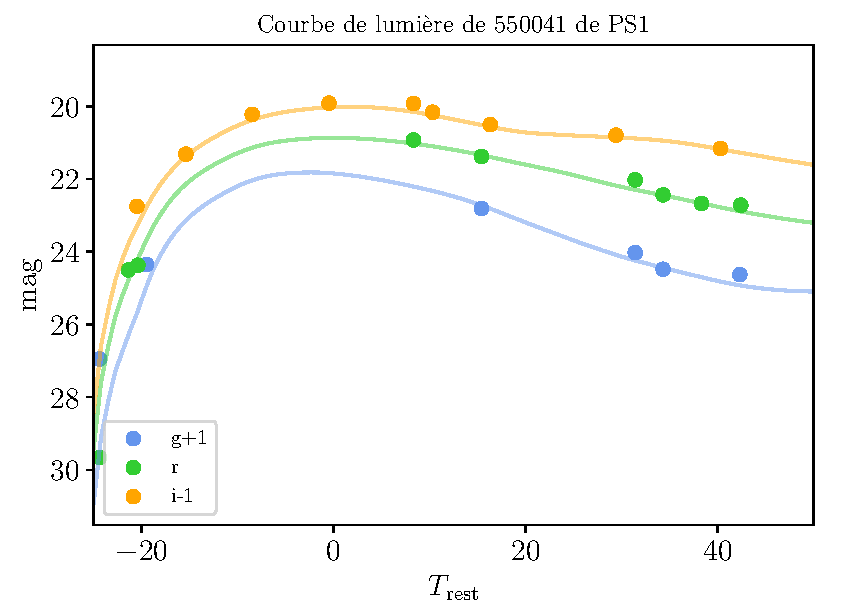
\includegraphics[width=\linewidth]{lc_550041.pdf}
        \captionsetup{justification=centering}
        \caption{Courbe de lumière en bandes $gri$ de la SN Ia confirmée 550041,
        à $z = 0,26$.}
        \label{fig:lc_550041}
    \end{subfigure}
    \caption{Caractéristiques du sondage PS1.}
\end{figure}

\subsubsection{Suivi spectro-photométrique}\label{sssec:ps1spectro}

Comme SDSS, PS1 utilise de nombreux différents instruments pour le suivi
spectroscopique~: le \textit{Blue Channel Spectrograph}~\citep{schmidt1989} et
le \textit{Hectospec}~\citep{fabricant2005} sur le télescope MMT de \SI{6,5}{m},
les spectrographes de \textit{Gemini Multi-Object Spectrographs}
\citep[GMOS,][]{hook2004}, le \textit{Low Dispersion Survey Spectrograph-3}
(LDSS3\footnote{\href{http://www.lco.cl/telescopes-information/magellan/instruments-1/ldss-3-1}
{http://www.lco.cl/telescopes-information/magellan/instruments-1/ldss-3-1}}) et
le \textit{Magellan Echellette}~\citep[MagE,][]{marshall2008} sur le télescope
\textit{Magellan Clay} de \SI{6,5}{m}, le \textit{Inamori-Magella Areal Camera
and Spectrograph}~\citep[IMACS,][]{dressler2011} sur le télescope
\textit{Magellan Baade} de \SI{6,5}{m}, le spectrographe ISIS sur le
WHT\footnote{\href{http://www.ing.iac.es/PR/wht_info/whtisis.html}
{http://www.ing.iac.es/PR/wht\_info/whtisis.html}} de \SI{4,2}{m}, et le DEIMOS
\citep{faber2003} sur le Keck de \SI{10}{m}~\citep{oke1995}.

Les critères les plus importants pour la sélection de candidats à observer
spectroscopiquement sont la position et la luminosité~: \textit{Magellan} et
\textit{Gemini} ne peuvent pointer que 5 des 10 champs du MDS, et certains
appareils ne peuvent acquérir des données qu'à $r_{\rm P1} \lesssim
\SI{21,5}{mag}$. La quantité de données observées par PS1 a souffert d'un manque
d'accès aux télescopes, de mauvais temps et de maintenance, réduisant
l'efficacité de suivi. L'évolution de ce paramètre en fonction de la magnitude
est donnée Figure~\ref{fig:speceff}. En résumé, la limite de détection pour
identifier les phénomènes transitoires produit des courbes de lumière de qualité
pour les SNe~Ia de $m < 24$, alors que l'échantillon spectroscopique est
principalement constitué d'objets de $m < 22$. Au total, ce sont 365 SNe~Ia
confirmées qui constituent l'échantillon de PS1.

\subsubsection{Données conservées}\label{ssec:ps1data}

Comme pour SDSS, pour une analyse cosmologique de qualité chaque SN~Ia se doit
d'avoir une courbe de lumière bien échantillonnée pour correctement contraindre
les paramètres d'optimisation, mais également que ses propriétés permettent de
limiter les biais systématiques dans la distance finale.
Ainsi,~\cite{scolnic2018} utilisent les coupes suivantes~:
\begin{enumerate}
    \item Optimisation donnant $\chi^2/\mathrm{NDOF} < 3,0$ (avec NDOF le nombre
        de degrés de liberté), réduisant le sondage à 332 données~;
    \item Erreur sur $x_1$ ($\s_{x_1}$) $< 1,0$, laissant 303 SNe~Ia~;
    \item Erreur sur le pic de magnitude ($\s_{\rm pkmjd}$) $< 2,0$, ne causant
        aucune coupe~;
    \item Paramètre de couleur $c$ tel que $-0,3 < c < 0,3$, rejetant 10 SNe~Ia
        pour 293 restantes~;
    \item Paramètre de stretch $x_1$ tel que $-3 < x_1 < 3$, que 5 SNe~Ia ne
        vérifient pas~;
    \item Extinction de la Voie Lactée $E(B-V)_{\rm MW}< \SI{0,20}{mag}$, ne
        s'appliquant pas aux données de PS1 grâce à la faible extinction des
        champs du MDS~;
    \item Au moins une mesure à $T_{\rm rest} > \SI{5}{jours}$, excluant 6
        SNe~Ia pour un total de 282 SNe~Ia.
\end{enumerate}
Une ultime coupe de l'analyse cosmologique par \textit{BEAMS with Bias
Correction}~\citep[BBC,][]{kessler2017} réduit cet échantillon à 279 données. La
méthode BBC impose que les propriétés d'une SN se retrouvent dans les 99.999\%
d'un échantillon simulé de 500 000 SNe du même sondage~; en l'occurrence les 3
SNe~Ia ne passant pas cette restriction ont pour paramètres $(x_1,c)$~:
$(−2,915, 0,083)$, $(−1,702, 0,271)$, et $(−0,893, 0,298)$. Ce procédé sera
discuté Chapitre~\ref{ch:snana}. La Table~\ref{tab:ps1cuts} résume cette
sélection, et la Figure~\ref{fig:ps1hist} présente les histogrammes en
redshifts, stretch et couleur de ces 279 données.

\begin{table}[]
    \centering
    \begin{threeparttable}
        \caption{Critères de sélection des SNe~Ia suivies par PS1.}
        \label{tab:ps1cuts}
        \begin{tabular}{lc}
            \toprule
            Critères de sélection     & Nb de SNe~Ia \\
            \midrule
            Confirmées                & 365 \\
            Courbe de lumière         & 332 \\
            $\s_{x_1} < 1$            & 303 \\
            $\s_{\rm pkmjd} < 2$      & 303 \\
            $-0,3 < c < 0,3$          & 293 \\
            $-3 < x_1 < 3$            & 288 \\
            $E(B-V)_{\rm MW} < 0,20 $ & 288 \\
            $T_{\max} > 5$            & 282 \\
            \midrule
            Coupe par BBC             & 279 \\
            \bottomrule
        \end{tabular}
        \begin{tablenotes}[flushleft]
        \item \textbf{\hspace{-3,2pt}Notes.} Le nombre de SNe est tiré de
            l'analyse de Pantheon.
        \end{tablenotes}
    \end{threeparttable}
\end{table}

\begin{figure}[ht]
    \centering
    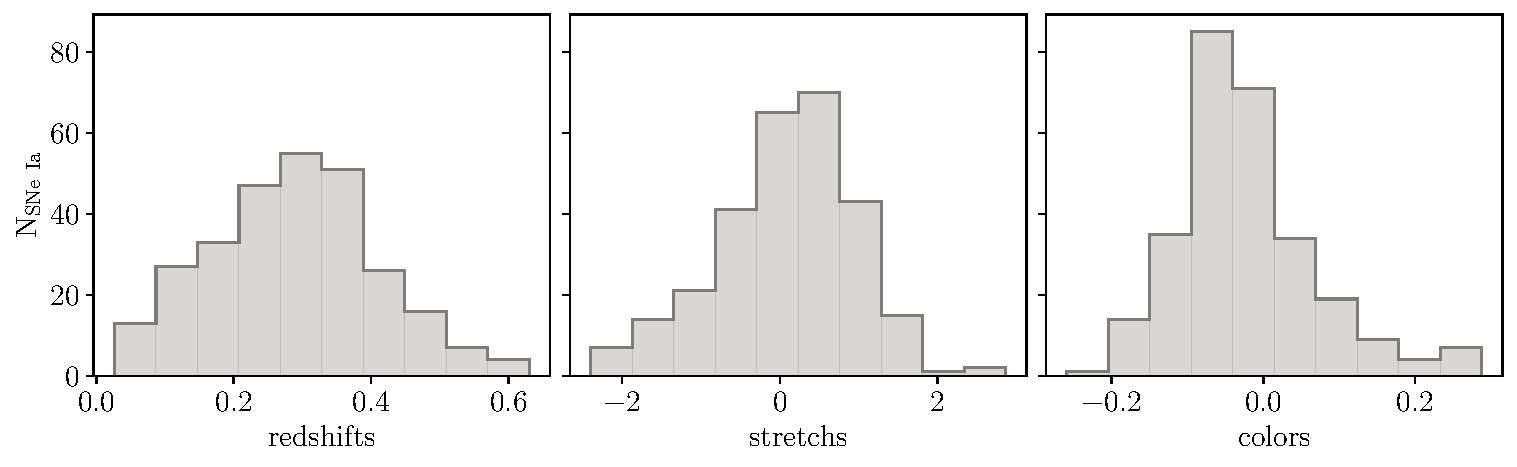
\includegraphics[width=\linewidth]{hist_PS1_zxc.pdf}
    \captionsetup{justification=centering}
    \caption{Distributions des paramètres de redshift (à gauche), de stretch (au
    milieu) et de couleur (à droite) pour les 279 données de PS1.}
    \label{fig:ps1hist}
\end{figure}

\subsection{SuperNovae Legacy Survey}\label{ssec:snls}
\subsubsection{Introduction}\label{sssec:snlsintro}

Le \textit{Supernova Legacy Survey}~\citep[SNLS,][]{astier2006, sullivan2011}
est un programme astronomique s'étendant sur 5 ans entre 2003 et début 2009,
dont le but principal est de mesurer l'expansion de l'Univers à l'aide de SNe~Ia
\textit{via} la mesure du paramètre d'état de l'énergie sombre $w$ à 5\% de
précision statistique et 10\% en incluant les effets systématiques. Il a été
conçu dans le but d'améliorer significativement les sondages passés grâce à sa
recherche glissante d'une part, mais également grâce à l'exploitation du service
d'observation à la fois pour la photométrie et la spectroscopie, réduisant
l'impact du mauvais temps. L'utilisation d'un seul instrument d'imagerie pour
observer les mêmes champs réduit les incertitudes systématiques photométriques ;
l'observation de service optimise à la fois le rendement du temps d'observation
spectroscopique et l'échantillonnage de la courbe de lumière.

\subsubsection{Détection des supernovae}\label{sssec:snlsdetec}

SNLS utilise la caméra MegaCam~\citep{boulade2003}, associée au télescope
Canada-France-Hawaï\footnote{\href{https://www.cfht.hawaii.edu/}
{https://www.cfht.hawaii.edu/}}, en se concentrant sur la partie profonde du
CFHTLS\footnote{\href{https://www.cfht.hawaii.edu/Science/CFHTLS/}
{https://www.cfht.hawaii.edu/Science/CFHTLS/}} représentant \SI{4}{deg^2} du
ciel réparti sur 4 champs de \SI{1}{deg^2} chacun et à faible extinction
galactique. L'acquisition se fait en 4 bandes $g'r'i'z'$ avec une cadence de
\SI{7}{jours} et une profondeur de \SI{25,0}{mag} en bande
$r$\footnote{\href{https://www.cfht.hawaii.edu/Science/CFHTLS/cfhtlsfinalreleaseexecsummary.html}
{https://www.cfht.hawaii.edu/Science/CFHTLS/cfhtlsfinalreleaseexecsummary.html}}
(et \SI{25,5}{mag} en bande $g$). Le système de filtre de SNLS est similaire à
celui de SDSS (cf. Section~\ref{ssec:sdss}), mais la spécificité de SNLS est de
pouvoir correctement mesurer la couleur de toutes les SNe~Ia sur la majeure
partie de l'intervalle de redshifts sondés grâce à ses 4 filtres permettant
d'intégrer les corrections $K$ aux mesures (contre la restriction aux bandes
$gri$ de SDSS). Les transmissions des filtres sont tracées
Figure~\ref{fig:snlsbands}, et un exemple de courbe de lumière est donné
Figure~\ref{fig:snlslc}

\begin{figure}[ht]
    \centering
    \begin{subfigure}[]{.49\linewidth}
        \centering
        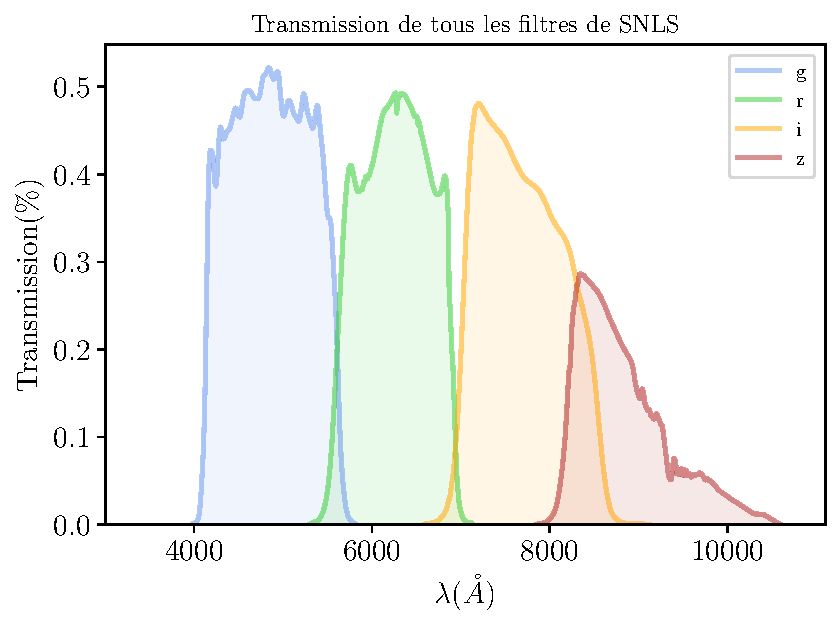
\includegraphics[width=\linewidth]{bands_SNLS.pdf}
        \captionsetup{justification=centering}
        \caption{Transmissions des filtres de MegaCam utilisés par SNLS.}
        \label{fig:snlsbands}
    \end{subfigure}
    \begin{subfigure}[]{.49\linewidth}
        \centering
        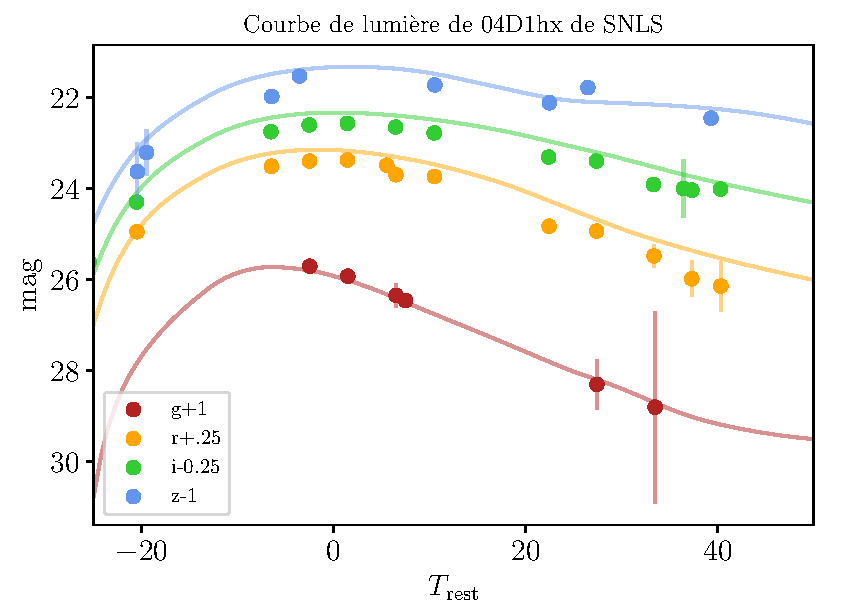
\includegraphics[width=\linewidth]{lc_04D1hx.pdf}
        \captionsetup{justification=centering}
        \caption{Courbe de lumière en bandes $griz$ de la SN~Ia confirmée
        04D1hx, à $z = 0,56$.}
        \label{fig:snlslc}
    \end{subfigure}
    \caption{Caractéristiques du sondage SNLS.}
\end{figure}

\subsubsection{Suivi spectro-photométrique}\label{sssec:snlsspectro}

Par la profondeur de son acquisition, SNLS utilise des télescopes dont les
miroirs ont un diamètre entre 8 et \SI{10}{m}~: le Keck~\citep{oke1995,
ellis2008}, le Very Large Telescope \citep[VLT,][]{balland2009} et les
télescopes Gemini~\citep{hook2004} pour le typage et la détermination du
redshift. Toutes les données de SNLS doivent être confirmées
spectroscopiquement. La partie photométrique du sondage délivrant plus de
candidats qu'il n'est possible d'observer spectroscopiquement, un classement des
phénomènes transitoires a dû être effectuer. Ce classement est déterminé en vue
d'optimiser le rendement en SNe~Ia, et utilise à la fois un outil de sélection
photométrique réalisant un ajustement de courbe de lumières en temps réel pour
éviter la contamination avec d'autres types de SNe~Ia, mais utilise également
une base de données de tous les phénomènes transitoires observés pour écarter
les étoiles variables qui varient sur de longs temps (plus d'une année). Les
candidats les moins lumineux, $i > \SI{24,5}{mag}$ (probablement à $z > 1$) et
ceux dont la luminosité n'est que faiblement supérieure à celle de leur galaxie
hôte (complexifiant l'identification) ne sont pas observés~: avec cette méthode,
environ 70\% des candidats observés se sont avérés être des SNe~Ia. Sur la
totalité de l'existence de ce sondage, ce sont 242 supernovae qui ont été
suivies et confirmées. L'efficacité spectroscopique du sondage est tracée
Figure~\ref{fig:speceff}.

\subsubsection{Données conservées}\label{ssec:snlsdata}

Toujours suivant~\cite{scolnic2018}, les données conservées répondent aux coupes
mentionnées Section~\ref{ssec:ps1}, les mêmes que pour PS1. L'échantillon final
se compose alors de 236 SNe~Ia. Une présentation graphique des données en
redshift, stretch et couleur de ces données est présentée
Figure~\ref{fig:snlshist}.

\begin{figure}[ht]
    \centering
    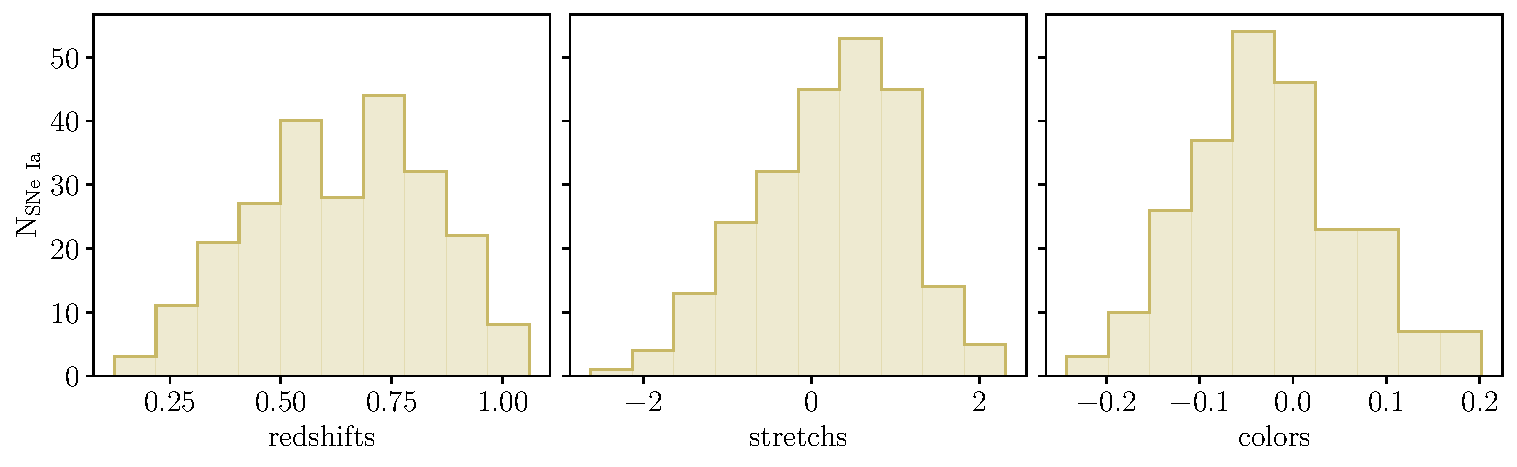
\includegraphics[width=\linewidth]{hist_SNLS_zxc.pdf}
    \captionsetup{justification=centering}
    \caption{Distributions des paramètres de redshift (à gauche), de stretch (au
    milieu) et de couleur (à droite) pour les 236 données de SNLS.}
    \label{fig:snlshist}
\end{figure}

\subsection{\textsc{Hubble} Space Telescope}\label{ssec:hst}

Plusieurs sondages permettant l'acquisition de données de SNe~Ia ont été
effectués avec le télescope spatial \textsc{Hubble}
(HST\footnote{\href{https://www.nasa.gov/mission_pages/hubble/story/index.html}
{https://www.nasa.gov/mission\_pages/hubble/story/index.html}})~: le
\textit{Great Observatories Origins Deep
Survey}~\citep[GOODS,][]{giavalisco2004, strolger2004, riess2007}, le
\textit{Supernova Cosmology Project} \citep[SCP,][]{suzuki2012}, et les sondages
\textit{Cosmic Assembly Near-infrared Deep Extragalactic Legacy
Survey}~\citep[CANDELS,][]{rodney2014} et \textit{Cluster Lensing And Supernova
Survey with Hubble}~\citep[CLASH,][]{graur2014}. Tous ces sondages recueillent
des données à $z > 1$ qui se révèlent d'une grande importance par leur poids
dans le diagramme de \textsc{Hubble} pour tester l'évolution des propriétés des
SNe. Ils sont combinés par la suite sous le nom «~HST~»~; ainsi, par souci
d'efficacité, nous ne détaillons ici que les résultats issus de GOODS qui
constituent la plus grande part des données à haut redshift de notre
échantillon.

\subsubsection{Introduction}\label{sssec:hstintro}

Le sondage \textit{\textsc{Hubble} Higher $z$ Supernova
Search}~\citep[HHZSS,][]{strolger2004}, sous-programme de GOODS, est un des
premiers sondages de recherche de SNe depuis l'espace. Son but principal est
d'étudier la présence de biais astrophysiques rendant les SNe~Ia intrinsèquement
moins lumineuses avec la distance, imitant une preuve de l'existence de
l'énergie sombre. Ce programme vise à relever des données au-delà de $z = 1$,
entre $1 < z < 2$. Dans cette plage, les SNe~Ia devraient exploser à une époque
de décélération cosmique, devenant ainsi relativement plus brillantes qu'à des
décalages vers le rouge plus faibles. On s'attend à ce que cela se distingue
clairement des simples effets de mesure astrophysiques, permettant une meilleure
connaissance des SNe~Ia. Étudier de manière approfondie et fiable ces SNe~Ia et
réaliser les observations de suivi nécessaires pour une telle étude nécessite
des observations plus profondes que ce qui peut être réalisé avec des télescopes
terrestres. Les observations de ce sondage s'étendent sur une plage
\SI{8}{mois}.

\subsubsection{Détection des supernovae}\label{sssec:hstdetec}

Ce programme utilise la \textit{Advanced Camera for
Surveys}\footnote{\href{https://www.nasa.gov/content/hubble-space-telescope-advanced-camera-for-surveys}
{https://www.nasa.gov/content/hubble-space-telescope-advanced-camera-for-surveys}}
(ACS). GOODS combine des observations multibandes extrêmement profondes de
l'ultraviolet à l'optique (dans le référentiel au repos) par le biais des
filtres F435W, F606W, F775W et F850LP, avec une magnitude limite pour F850LP
$\approx$ 26. Deux champs ont été observés pour une
surface totale d'acquisition de \SI{300}{arcmin^2}, chacun à haute latitude
écliptique pour permettre aux opérations au sol d'observer depuis les deux
hémisphères. Sa cadence est d'environ \SI{45}{jours}, suffisante pour détecter
les SNe~Ia vers le maximum d'émission pour $z \approx 1$ et avant le maximum
pour $z > 1,3$ (dû à l'étalement de la courbe de lumière du fait de
l'expansion~; dans le référentiel au repos le temps de montée typique est de
$\approx \SI{20}{jours}$), mais permet également de s'assurer qu'une SN
dépassant le seuil de détection ne repasse pas en-dessous avant seconde
observation. Les transmissions des filtres utilisés par le sondage sont tracées
Figure~\ref{fig:hstbands}.

\begin{figure}[!ht]
    \centering
    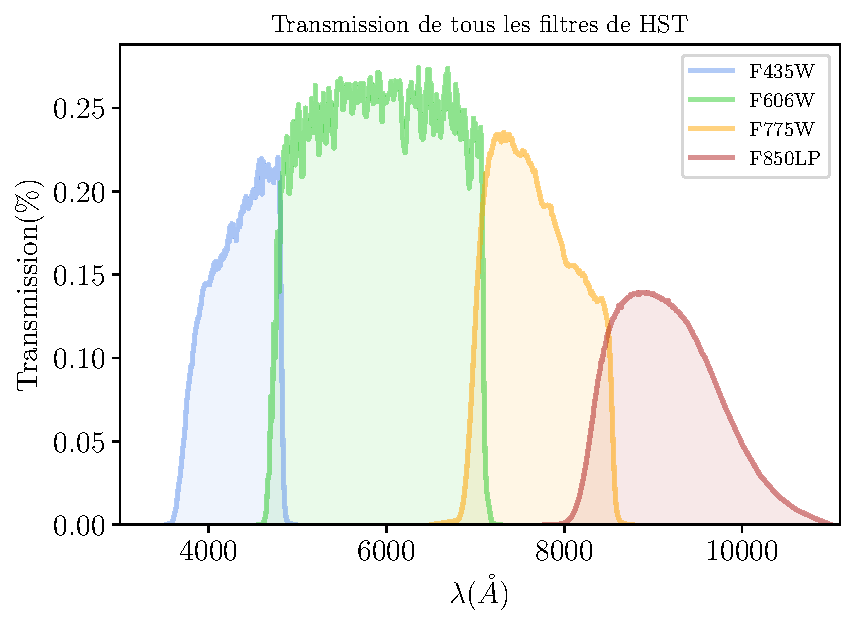
\includegraphics[width=.6\linewidth]{bands_HST.pdf}
    \captionsetup{justification=centering}
    \caption{Transmissions des filtres de ACS utilisés par HST.}
    \label{fig:hstbands}
\end{figure}

\subsubsection{Suivi spectro-photométrique}\label{sssec:hstspectro}

Le HST, grâce à sa présence dans l'espace notamment, permet de produire des
spectres avec un rapport signal sur bruit significativement supérieur à ce qu'il
est possible d'atteindre par rapport à un instrument au sol. Il est cependant
limité par sa faible résolution spectrale et le recouvrement de multiples ordres
spectraux d'autres sources proches~: ainsi, seules les SNe avec un séparation
angulaire notable avec leur hôte et d'autres sources lumineuses ont été
observées. Une méthode secondaire d'identification des SNe~Ia par photométrie a
été utilisée pour optimiser la confirmation spectroscopique. \cite{riess2007}
détaillent les données ayant la plus haute qualité, qualifiées de «~dorées~»~:
celles dont la classification est certaine (rapport signal sur bruit $\gtrsim$
20) et dont la photométrie est suffisante pour amener à une estimation de
distance robuste, facilement caractérisée par les erreurs de mesure. On relève
42 données de~\cite{strolger2004} et 21 de~\cite{riess2007}.

\subsubsection{Données conservées}\label{sssec:hstdata}

À ces distances, le typage peut s'avérer difficile mais la classification des
données «~dorées~» est suffisamment robuste pour les inclure dans l'analyse
cosmologique de~\citep{scolnic2018}~; ces données ne sont donc pas sujettes à
d'autres coupes. En combinant SCP, GOODS, CLASH et CANDELS, ce sont 26 données
qui constituent l'échantillon HST~; le détail des données par sondage est
indique Table~\ref{tab:hstcuts}, et la distribution des paramètres en redshift,
stretch et couleur est montrée Figure~\ref{fig:hsthist}.

\begin{table}[]
    \centering
    \begin{threeparttable}
        \caption{Nombre de SNe~Ia composant notre échantillon HST selon les
        sondages à haut redshifts.}
        \label{tab:hstcuts}
        \begin{tabular}{lcc}
            \toprule\toprule
            Sondage & Nb de SNe~Ia & $z$ moyen \\
            \midrule
            SCP     & 3            & 1,092 \\
            GOODS   & 15           & 1,120 \\
            CLASH   & 2            & 1.555\\
            CANDELS & 6            & 1,732 \\
            \midrule
            Total   & 26           & \\
            \bottomrule
        \end{tabular}
        \begin{tablenotes}[flushleft]
        \item \textbf{\hspace{-3,2pt}Notes.} Le nombre de SNe est tiré de
            l'analyse de Pantheon.
        \end{tablenotes}
    \end{threeparttable}
\end{table}

\begin{figure}[]
    \centering
    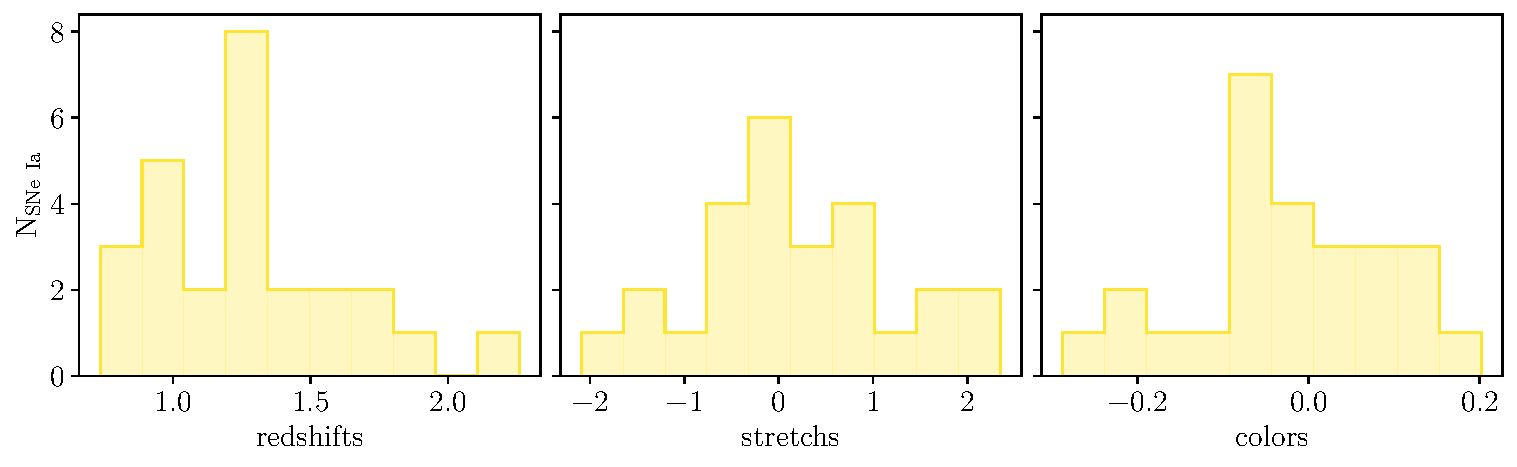
\includegraphics[width=\linewidth]{hist_HST_zxc.pdf}
    \captionsetup{justification=centering}
    \caption{Distributions des paramètres de redshift (à gauche), de stretch (au
    milieu) et de couleur (à droite) pour les 26 données de HST.}
    \label{fig:hsthist}
\end{figure}

\subsection{Autres sondages~: CfA1-4 et CSP}\label{ssec:lowz}

Enfin, bien que ces sondages n'apparaissent pas dans la première partie de cette
étude, nous utilisons d'autres données à bas redshifts que celles issues de
SNfactory. Comme pour la section précédente, ces données proviennent d'une
combinaison de sondages~: celles des 4 relevés du \textit{Center for
Astrophysics} de Harvard, nommés CfA1 à 4~\citep{riess1999, jha2006,
hicken2009a, hicken2009b, hicken2012} et des 2 publications du \textit{Carnegie
Supernova Project}~\citep[CSP,][]{contreras2010, folatelli2010,
stritzinger2011}. Ils ne feront pas l'objet de plus de détail avant le chapitre
pertinent (Chapitre~\ref{ch:snana}), étant donné que ce sont tous les sondages à
recherche ciblée que l'on écarte de notre échantillon. Cette combinaison de
sondage, résultant en 172 SNe~Ia après les coupes de~\cite{scolnic2018}, est
appelée \textit{LOWZ}, leur données s'étalant entre $0,01 < z < 0,07$. Une
présentation de leurs distributions de paramètres en redshift, stretch et
couleur est cependant donnée Figure~\ref{fig:lowzhist}.

\begin{figure}[ht]
    \centering
    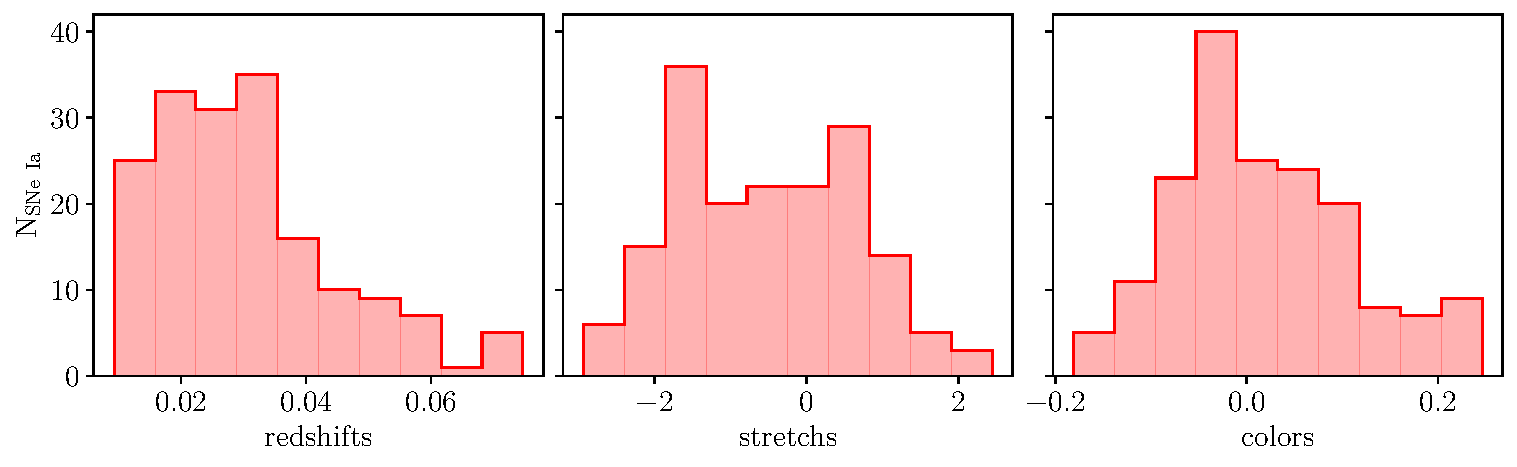
\includegraphics[width=\linewidth]{hist_LOWZ_zxc.pdf}
    \captionsetup{justification=centering}
    \caption{Distributions des paramètres de redshift (à gauche), de stretch (au
    milieu) et de couleur (à droite) pour les 172 données de LOWZ.}
    \label{fig:lowzhist}
\end{figure}

\subsection{Résumé et comparaison}\label{ssec:sondcomp}

Pour permettre une meilleure visualisation des diverses caractéristiques des
sondages traités dans cette thèse, nous présentons Table~\ref{tab:sondcomp} une
comparaison des éléments que nous considérons comme principaux dans ces
sondages.

\begin{table}[ht]
    \centerfloat
    \begin{threeparttable}
        \caption{Comparaison des caractéristiques des sondages utilisés.}
        \label{tab:sondcomp}
        \begin{tabular}{lcccccc}
            \toprule
            Sondage              &
            Surface (deg$^2$)    & Cadence (jours)   & Filtres          &
            Profondeur (mag)     & Intervalle $z$    & $N_{\rm SN}$\\
            \midrule
            \hyperref[ssec:snf]{SNf} &
            500                      & 1                 & BR               &
            $r \lesssim 19,5$        & $0,02 < z < 0,08$ & 114\\
            \hyperref[ssec:lowz]{LOWZ}\tnote{1}            &
            --                       & --                & $UBVRI$          &
            --                       & $0,01 < z < 0,07$ & 172\\
            \hyperref[ssec:sdss]{SDSS}                     &
            300                      & 4                 & $ugriz$          &
            $r \lesssim 22,5$        & $0,04 < z < 0,40$ & 335\\
            \hyperref[ssec:ps1]{PS1}                      &
            70                       & 7                 & $grizy_{\rm P1}$ &
            $r \lesssim 23,1$        & $0,03 < z < 0,63$ & 279\\
            \hyperref[ssec:snls]{SNLS}                     &
            4                        & 7                 & $g'r'i'z'$       &
            $r \lesssim 25,0$        & $0,13 < z < 1,06$ & 236\\
            \hyperref[ssec:hst]{HST}\tnote{1}             &
            0,08                     & 45                & $griz$\tnote{2}  &
            F850LP $\lesssim 26$     & $0,74 < z < 2,26$ & 26\\
            \midrule
            Total & \multicolumn{5}{c}{--} & 1162\tnote{3}\\
            \bottomrule
        \end{tabular}
        \begin{tablenotes}[flushleft]
        \item \textbf{\hspace{-3,2pt}Notes.} Le nombre de SNe est tiré de
            l'analyse de Pantheon.
        \item [1] Caractéristiques non pertinentes en temps que sondages ciblés.
        \item [2] Caractéristiques pour GOODS, intervalle et nombre de SNe~Ia
            pour tous les sondages HST.
        \item [3] Relativement équivalent, cf. Figure~\ref{fig:hstbands}.
        \item [4] 1048 sans SNf \citep{scolnic2018}, 990 sans LOWZ (base de
            notre échantillon).
        \end{tablenotes}
    \end{threeparttable}
\end{table}

Au travers des sections précédentes, nous avons pu avoir un aperçu de la
complexité que représente les relevés cosmologiques. La variété des intervalles
de redshifts et donc des caractéristiques des sondages impose des instruments
variés, des stratégies spécifiques, mais également des calibrations différentes.
Travailler avec de nombreux \NN{pipelines} d'analyse rend la combinaison de
sondages fastidieuse. C'est cet aspect que les prochains grands relevés
cosmologiques tentent d'améliorer~: le sondage \textit{Vera Rubin Observatory},
\textit{via} le \textit{Large Synoptic Survey Telescope}
\citep[LSST,][]{ivezic2019}, a pour objectif de couvrir un intervalle de
redshifts extrêmement grand, et le sondage de la \textit{Zwicky Transient
Facility}~\citep[ZTF,][]{bellm2019, dekany2020} répond aux difficultés
particulières de la partie à faible redshift de la cosmologie. On présente
Figure~\ref{fig:speceff} les différentes efficacités spectroscopiques avec le
redshifts des 4 sondages LOWZ, SDSS, PS1 et SNLS~: bien que les magnitudes
limites de ces programmes permettent de détecter des SNe~Ia à hauts redshifts,
la qualité de ces dernières se voit contrainte par les capacités de typage.
C'est cet aspect de la combinaison que nous traitons dans la partie suivante.

\begin{SCfigure}[0,5][h!]
    \centering
    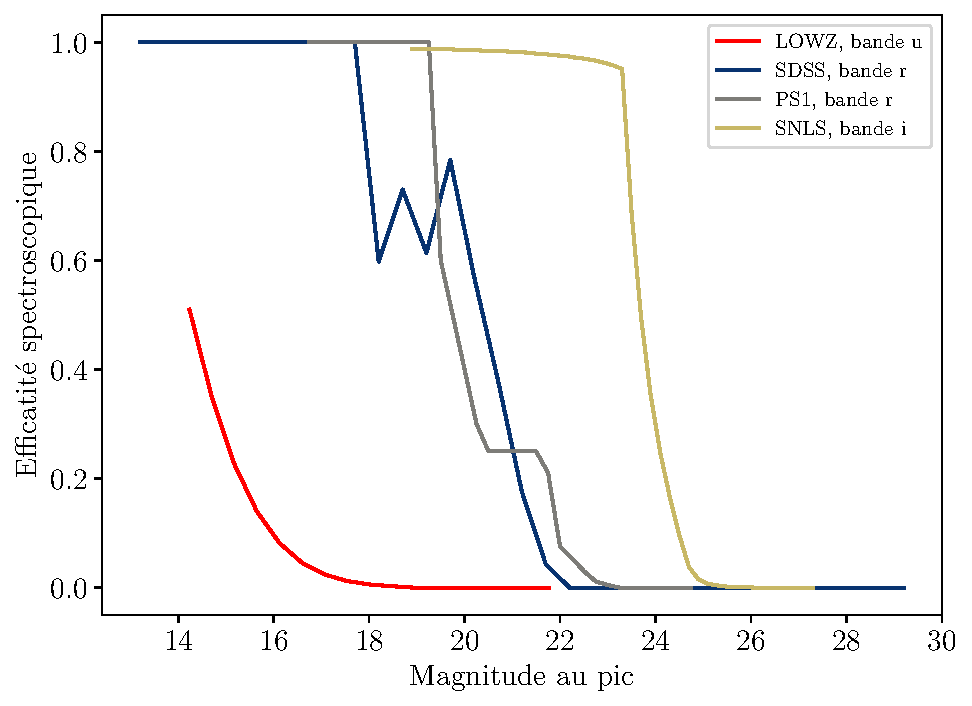
\includegraphics[width=.5\linewidth]{speceff-all.pdf}
    % \captionsetup{justification=centering}
    \caption{Comparaison des efficacités spectroscopiques des différents
    sondages.}
    \label{fig:speceff}
\end{SCfigure}

\section{Échantillon d'étude}\label{sec:sample}

Nous détaillons dans cette Section la procédure de construction de notre
échantillon volume-limité comme expliqué partie~\ref{ssec:malm}. Notre étude se
base sur les données de la combinaison de sondage Pantheon~\citep{scolnic2018},
en remplaçant la combinaison ciblée LOWZ par les données SNfactory dont la
sélection est maîtrisée et permettant une étude de sous-population grâce au
LsSFR. Les données de HST étant complètes, la confection de notre échantillon se
concentre sur les sondages SDSS, PS1 et SNLS~; leur nature non-ciblée et limitée
en magnitude permet d'en construire une portion limitée en volume comme décrit
Section~\ref{sec:compl}.

\subsection{Confection}\label{ssec:cuts}

Nous détaillons ici deux des approches mises en place visant à déterminer la
portion des sondages que l'on peut considérer limitées en volume.

\subsubsection{Approche statistique}\label{sssec:baserate}

À partir des données publiées dans~\cite{scolnic2018}\footnote{\href{
    https://archive.stsci.edu/hlsps/ps1cosmo/scolnic/data_fitres/}
{https://archive.stsci.edu/hlsps/ps1cosmo/scolnic/data\_fitres}}, il est
possible de tracer l'histogramme des SNe~Ia en fonction du redshift (cf.
Sections précédentes, par exemple Figure~\ref{fig:snfhist}, à gauche). En
supposant une densité volumique de supernovae uniforme, chaque intervalle de
redshift comprend un volume de plus en plus grand et on s'attend donc à observer
toujours plus de SNe~Ia avec la distance. On observe cependant une baisse de ce
nombre à partir d'un certain redshift. La chute de nombre de SNe~Ia provient de
cette limitation du sondage à mesurer la luminosité. Notre première approche a
été de se baser sur une étude statistique pour essayer de récupérer la valeur
estimée à partir de laquelle chaque sondage s'écarte d'un modèle volumétrique.
Le protocole est le suivant~:
\begin{itemize}
    \item Les bornes minimales et maximales des données sont augmentées d'une
        faible valeur aléatoire (entre 0,06 et 0,12 à gauche et entre 1,10 et
        1,15 à droite, pour SNLS) afin d'assurer une variation du centre des
        intervalles~;
    \item On choisit aléatoirement entre 5 et 20 intervalles pour tracer
        l'histogramme~;
    \item On initialise un modèle volumétrique $a\times
        \left(V(z_2)-V(z_1)\right)$ avec $a$ la densité volumique de SNe~Ia,
        paramètre libre du modèle, auquel on passe comme donnée les bords des
        intervalles.
    \item Les valeurs du modèle sont comparées aux hauteurs des intervalles de
        l'histogramme, permettant l'ajustement du modèle par une loi de Poisson
        cumulée~\citep[voir par exemple][]{syed2015}. Pour un intervalle donné
        de nombre moyen de données $\lambda$, la probabilité qu'il y en ait
        exactement $k$ est, d'après la loi de Poisson~:
        \begin{equation}\label{eq:poisson}
            p(k) = \mathcal{P}(X = k) = \frac{\lambda^k}{k!}e^{-\lambda}
        \end{equation}
        La fonction de répartition, ou de distribution cumulative, est donnée
        par~:
        \begin{equation}\label{eq:pcdf}
            \mathcal{P}(X\leq x) = \sum_{k=0}^{x}p(k) = e^{-\lambda}
            \sum_{k=0}^{x} \frac{\lambda^k}{k!}
        \end{equation}
    \item On choisit aléatoirement un intervalle maximal après lequel
        l'ajustement s'arrête, avec un minimum de 3 intervalles (6 dans les cas
        des Figures de~\ref{fig:zmax_method}), 10 fois pour chaque histogramme~;
    \item On sauve les positions et valeurs de probabilité des intervalles
        ajustés et créé une interpolation linéaire des résultats~;
    \item Ces 5 étapes sont répétées 1000 fois et on calcule la médiane et
        l'écart type des 10 000 interpolations calculées.
\end{itemize}

\begin{figure}[ht]
    \centering
    \begin{subfigure}[]{.49\linewidth}
        \centering
        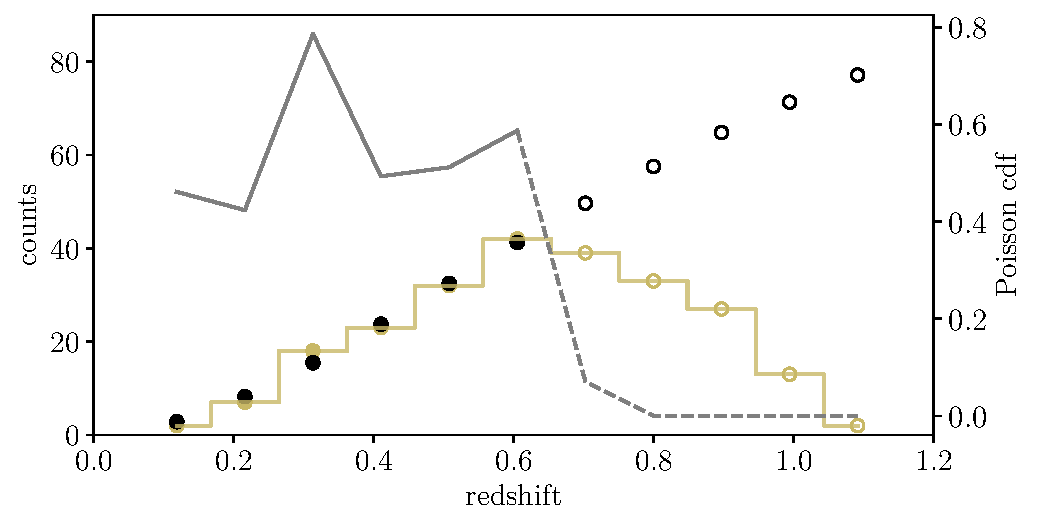
\includegraphics[width=\linewidth]{zmax_method_snls-01.pdf}
        \captionsetup{justification=centering}
        \caption{11 intervalles, ajustement sur 6}
        \label{fig:zmax_method1}
    \end{subfigure}
    \begin{subfigure}[]{.49\linewidth}
        \centering
        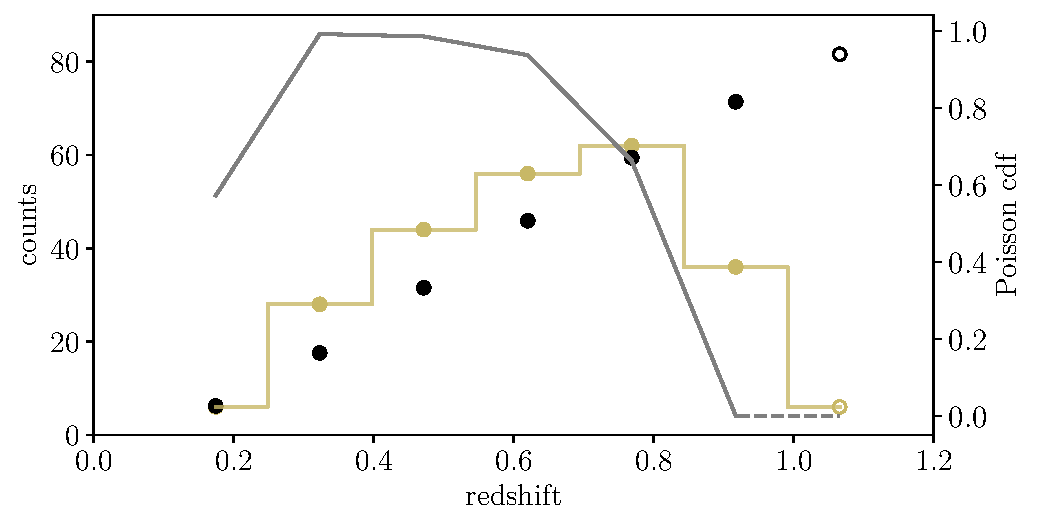
\includegraphics[width=\linewidth]{zmax_method_snls-02.pdf}
        \captionsetup{justification=centering}
        \caption{7 intervalles, ajustement sur 6}
        \label{fig:zmax_method2}
    \end{subfigure}
    \captionsetup{justification=centering}
    \caption{Exemple d'ajustement statistique pour deux tirages aléatoires
    d'histogrammes de SNLS}
    \label{fig:zmax_method}
\end{figure}

% Deux modèles ont été testés. Le premier est issu de \textbf{perrett2012} donnant
% un taux volumétrique co-mobile~:
% \begin{equation}\label{eq:perrett}
%     R(z) = 1.75\times10^{-5}(1+z)^{2,11}\,{\rm yr^{-1}Mpc^{-3}}
% \end{equation}
% Le second est directement issu du calcul d'un volume co-mobile dérivé des
% équations de la relativité générale~:

Le modèle volumétrique retenu dans notre analyse est défini par~:
\begin{equation}\label{eq:comobvol}
    V(z) = \frac{4\pi}{3}\times d_C{}^3(z)
\end{equation}
avec $d_C(z)$ la distance comobile
\begin{align}
    d_C(z)                           & =
    \frac{c}{H_0} \int_{0}^{z} \frac{\d z'}{E(z')}
    \quad\text{avec}\quad\\
    E(z) \triangleq \frac{H(z)}{H_0} & =
    \left[\Omega_R(1+z)^4 + \Omega_M(1+z)^3 +
        \Omega_k(1+z)^2 + \Omega_\Lambda
    \right]^{1/2}
\end{align}

On a choisi la cosmologie issue de la collaboration Planck~\citep{planck2018},
dont les valeurs sont indiqués Table~\ref{tab:planckvals}.

\begin{table}[ht]
    \centering
    \caption{Valeur des paramètres cosmologiques utilisés pour la détermination
    statistique du redshift limite des sondages SDSS, SNLS et PS1.}
    \label{tab:planckvals}
    \begin{tabular}{ccccc}
        \toprule
        $H_0$ &
        $\Omega_R$ & $\Omega_M$ & $\Omega_k$ & $\Omega_\Lambda$ \\
        \midrule
        \SI{67,74}{km.Mpc^{-1}.s^{-1}} &
        $5.389\times10^{-5}$ & 0,3075 & 0 & 0,6910 \\ 
        \bottomrule
    \end{tabular}
\end{table}

Le résultat de ces calculs donne une estimation du redshift à partir duquel
chacun des sondages n'a plus la capacité à recueillir toutes les SNe~Ia,
représentée Figure~\ref{fig:zmax_method_results}. En estimant $z_{\lim}$ comme
étant la valeur à laquelle la médiane des distributions cumulées chute à 0,5 et
les erreurs basse et haute à 0,525 et 0,475 respectivement, on obtient les
valeurs de la Table~\ref{tab:zlimsample}.

\begin{figure}[ht]
    \centering
    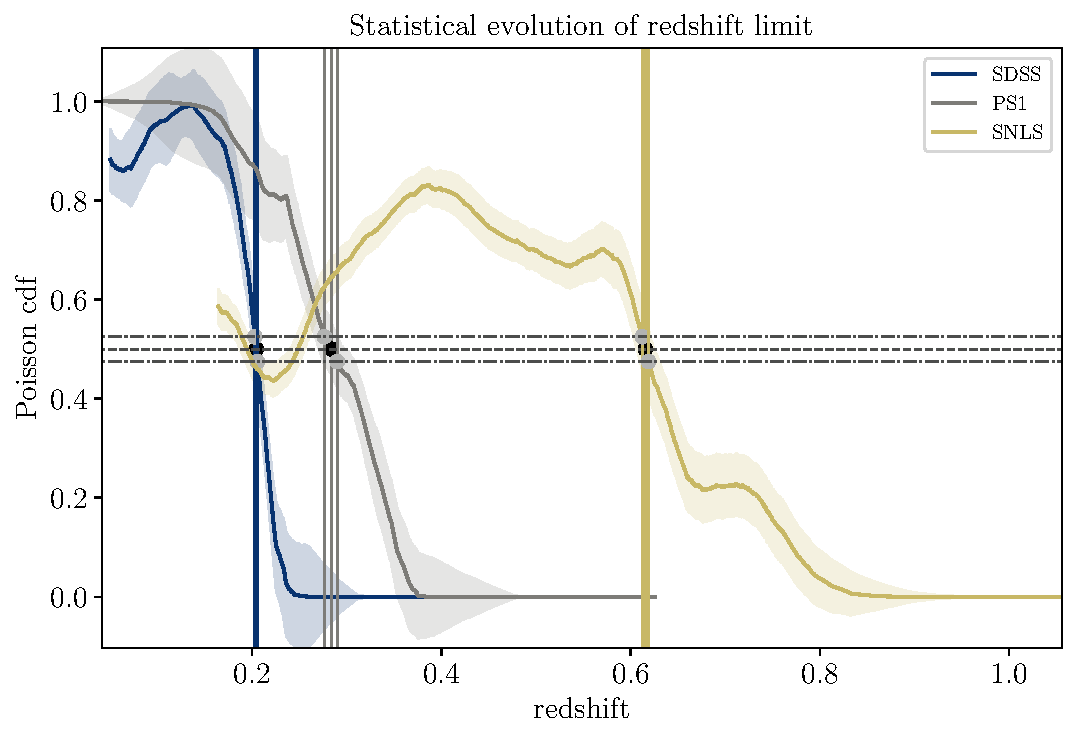
\includegraphics[width=.7\linewidth]{zmax_method_results.pdf}
    \captionsetup{justification=centering}
    \caption{Résultat graphique de l'évolution médiane de l'étude statistique du
    redshift limite pour les sondages SDSS, PS1, et SNLS}
    \label{fig:zmax_method_results}
\end{figure}

Cette première approche présente une robustesse certaine dans l'établissement
des évolutions statistiques en répétant le processus précédent. Cependant, le
sens de variation non constant du résultat de SNLS et de PS1 ne permettent pas
de forte confiance dans la correspondance de ce protocole au but de cette
étude~; de plus, le choix de la valeur de la fonction de répartition à laquelle
on peut considérer le sondage complet n'est pas motivée mathématiquement ou
physiquement de manière systématique. Cette conclusion nous a amenæ à une
approche combinant à la fois la réalité de la sélection astrophysique
instrumentale et les équations de distribution de luminosité de SN~Ia avec leurs
paramètres $x_1$, $c$ et $z$.

\subsubsection{Approche analytique}\label{sssec:maglim}

En supposant que ces sondages ont un typage spectroscopique et suivi
photométrique suffisant, ils devraient avoir des effets de sélection de
sous-population de SNe~Ia négligeables en deçà d'un certain redshift permettant
l'acquisition de toute la zoologie de stretch et couleur. Les données de SNe~Ia
issues de l'ajustement par \texttt{SALT2.4} ne contiennent que des données avec
un maximum de $x_1 = \pm 3$ et de $c = \pm 0,3$~\citep[][cf
Section~\ref{ssec:salt}]{guy2007, betoule2014}.

La magnitude absolue d'une supernova à son maximum de luminosité est, d'après
l'équation~\ref{eq:mxc}~:
\begin{equation*}
    M = M_0 -\alpha x_1 + \beta c
\end{equation*}
avec $M_0 = \SI{-19,36}{mag}$ dans le filtre photométrique $B$ de Bessell
\citep{kessler2009a, scolnic2014}, $\alpha=0,158$ et $\beta=3,14$
\citep[Table 7,][]{scolnic2018}. On détermine cette quantité sur l'ellipse
limite des paramètres grâce au paquet \texttt{sncosmo}
\footnote{\href{https://sncosmo.readthedocs.io/en/stable/}
{https://sncosmo.readthedocs.io/en/stable/}}, représentée par un gradient de
couleur Figure~\ref{fig:maglim}. On trouve alors que la supernova la moins
lumineuse est celle de paramètres $x_1 = -1,65$ et $c = 0,25$ dont le maximum de
magnitude absolue standardisée est $M_{\min}^{t_0}=\SI{-18,31}{mag}$.

\begin{figure}
    \centering
    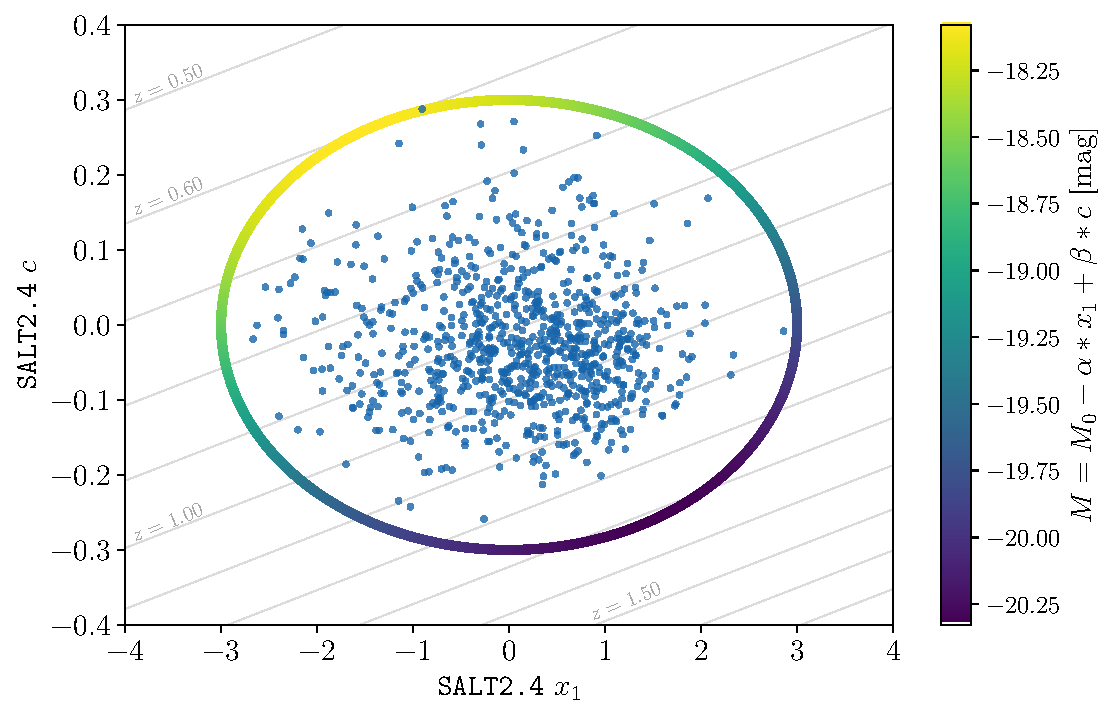
\includegraphics[width=0.95\linewidth]{zmax_maglim_snls.pdf}
    \caption[Distribution et limite des paramètres de courbe de lumière de
    stretch ($x_1$) et de couleur ($c$) des sondages SDSS, PS1 et SNLS combinés
    du catalogue Pantheon.]{Distribution des paramètres de courbe de lumière de
        stretch ($x_1$) et de couleur ($c$) issus d'un ajustement par
        \texttt{SALT2.4} pour les données de SNe~Ia des sondages SDSS, PS1 et
        SNLS combinés du catalogue Pantheon. Chaque supernova est représentée
        par un point bleu. L'ellipse limite des paramètres $(x_1=\pm3,
        c=\pm0,3)$ est représentée avec un gradient de couleur correspondant à
        la magnitude absolue standardisée en utilisant les valeurs
        de~\cite{scolnic2018} pour les coefficients $\alpha$ et $\beta$. Les
        lignes diagonales grises représentent l'évolution de $m = m_{\lim}$ en
        fonction de $z$ dans le plan $(x_1,c)$ entre $z=0,50$ et $z=1,70$ pour
    la magnitude limite $m_{\lim}=\SI{24,8}{mag}$ du sondage SNLS.}
    \label{fig:maglim}
\end{figure}

Cependant, pour établir une courbe de lumière, une supernova doit être observée
typiquement au moins 5 jours avant et une semaine après son pic de luminosité,
donnant une magnitude absolue limite effective d'approximativement $M_{\lim}
= \SI{-18,00}{mag}$. En connaissant les magnitudes limites de chaque sondage et
avec l'équation reliant le module de distance aux magnitudes observée et
absolue
\begin{equation}\label{eq:distmod}
    \mu(z) = m - M
\end{equation}
on peut déterminer le redshift limite $z_{\lim}$ en-delà duquel la SN~Ia la
moins lumineuse ne sera pas observée. On a ainsi défini un ensemble de redshifts
limites définissant un échantillon fiduciel en prenant la limite suggérée par
cette analyse.

Cependant, cette solution pourrait ne pas être optimale étant donné qu'elle
ignore les efficacités de suivi spectroscopiques pour les redshifts en-dessous
de $z_{\lim}$~; c'est pourquoi nous avons également déterminé un autre ensemble
de coupes définissant un échantillon «~conservatif~». Cet échantillon est plus
petit et donc sera statistiquement moins pertinent, mais également moins sujet
aux effets de sélection. Ainsi si l'évolution des propriétés des SNe~Ia avec le
redshift est encore sondable dans l'échantillon conservatif, il serait encore
plus présent dans un échantillon dont l'absence d'effets de sélection est
effectuée avec plus de précision que nos coupes en redshift.

\paragraph*{Pour SNLS} dont les supernovae sont typiquement entre $0,4 < z <
0,8$, la bande $B$ de Bessell dans un référentiel au repos correspond
approximativement à son filtre $i$, de magnitude limite à 5$\sigma$ de
\SI{24,8}{mag}\footnote{\href{
    https://www.cfht.hawaii.edu/Science/CFHTLS/cfhtlsfinalreleaseexecsummary.html}
{https://www.cfht.hawaii.edu/Science/CFHTLS/cfhtlsfinalreleaseexecsummary.html}}.
Ceci implique $z_{\lim} = 0,60$, en accord avec~\cite{neill2006, perrett2010},
et~\citep[Section~2,2]{conley2011}. D'autre part, la Figure~14
de~\cite{perrett2010}, suggère une plus basse limite à $z_{\lim} = 0,55$. Nous
avons donc choisi $z=0,60$ et $z=0,55$ comme redshifts limites de SNLS pour les
échantillons fiduciel et conservatif respectivement.

\paragraph*{De la même manière pour PS1} leurs SNe~Ia sont entre $0,2 < z <
0,4$~; la profondeur à 5$\sigma$ dans la bande $g$ est de \SI{23,1}{mag} d'après
\cite{rest2014} et mène à $z_{\lim}=0,31$, en correspondance avec la Figure~6
de~\cite{scolnic2018} par exemple. De manière conservative, cette figure
suggère une limite plus prononcée à $z_{\lim}=0,27$~; ces deux valeurs
constituent donc les redshifts limites de PS1 pour la partie fiducielle et
conservative, respectivement, de notre échantillon.

\paragraph*{Dans le même intervalle pour SDSS} la magnitude limite est de
\SI{22,5}{mag} d'après~\cite{dilday2008} et~\cite{sako2008}~; cette valeur 
impliquerait $z_{\lim}=0,24$, mais les sondages SDSS se sont confrontés à une
limitation dans leurs capacités spectroscopiques. Comme indiqué
dans~\cite{kessler2009a} Section~2, les données de la première année de SDSS ont
favorisé les SNe~Ia de magnitude $r < \SI{20,5}{mag}$ pour identification
spectroscopique, ce qui correspondrait à une coupe de redshift à 0,15. Le reste
du programme a bénéficié de meilleures ressources spectroscopiques
et~\cite{kessler2009a} et~\cite{dilday2008} font preuve d'une complétude
raisonnable jusqu'à $z=0,2$. La Figure~3 de~\cite{conley2011}, donnée
Figure~\ref{fig:sdssmalm} donnant l'évolution du biais de Malmquist en fonction
du redshift confirme ces hypothèses. En nous basant sur ces faits, on a choisi
$z_{\lim}=0,20$ et $z_{\lim}=0,15$ pour nos échantillons fiduciel et conservatif
respectivement.

\begin{SCfigure}[0,7]
    \centering
    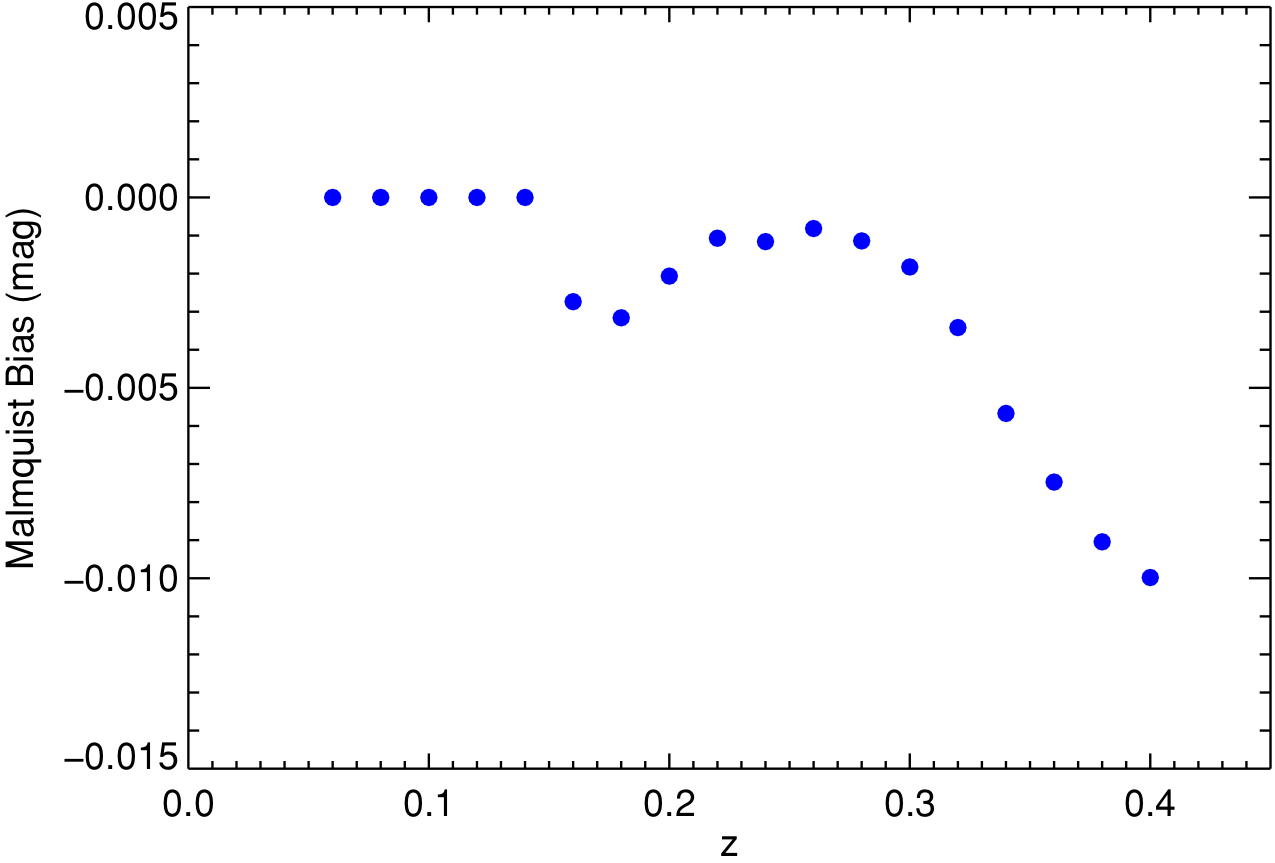
\includegraphics[width=.5\linewidth]{sdss_malquist.png}
    % \captionsetup{justification=centering}
    \caption[Biais de Malmquist moyen en fonction du redshift pour le sondage
    SDSS.]{Biais de Malmquist moyen en fonction du redshift pour le sondage
        SDSS. La forte baisse à $z=0,15$ est un artéfact dû à la discontinuité
        du modèle d'efficacité spectroscopique et n'a que peu d'effet sur les
    contraintes cosmologiques. Figure tirée de~\cite{conley2011}.}
    \label{fig:sdssmalm}
\end{SCfigure}

Cette approche est totalement systématique et reproductible, et donne des
$z_{\lim}$ similaires à l'approche statistique~; cette observation conforte donc
les résultats et choix de magnitudes limites, et ce sont ces résultats
analytiques que l'on a conservés dans notre étude. La comparaison des limites
par les deux méthodes et le nombre de données conservées avec les limites
analytiques dans les cas fiduciels et conservatifs sont indiqués
Table~\ref{tab:zlimsample}.

\begin{table}[ht]
    \centering
    \begin{threeparttable}
        \caption{Composition en SNe~Ia de notre échantillon.}
        \label{tab:zlimsample}
        \begin{tabular}{lccc}
            \toprule
            \multirow{2}[2]{*}{Sondage} &
            \multicolumn{2}{c}{$z_{\lim}$} &
            \multirow{2}[2]{*}{$N_{\rm SN}$}\\
            \cmidrule(lr){2-3}
            & Statistique & Analytique & \\
            \midrule
            SNf &
            \multicolumn{2}{c}{0,08} &
            114 \\
            SDSS & 
            0,204$^{+0,001}_{-0,001}$ & 0,20 (0,15) &
            167 (82) \\
            PS1 &
            0,284$^{+0,006}_{-0,008}$ & 0,31 (0,27) &
            160 (122) \\
            SNLS &
            0,615$^{+0,003}_{-0,003}$ & 0,60 (0,55) &
            102 (78) \\
            HST &
            \multicolumn{2}{c}{--} &
            26 \\
            \midrule
            Total & \multicolumn{2}{c}{--} &
            569 (422)\\
            \bottomrule
        \end{tabular}
        \begin{tablenotes}[flushleft]
        \item \textbf{\hspace{-3,2pt}Notes.} L'échantillon et notamment le
            nombre de SNe utilisées suivent les limites analytiques. Les nombres
            entre parenthèse correspondent aux limites conservatives.
        \end{tablenotes}
    \end{threeparttable}
\end{table}

\subsection{Présentation}\label{ssec:dataset}

Par rapport aux analyses cosmologiques générales, notre étude impose une forte
sélection sur des données déjà soigneusement choisies~: seulement 43\% (SNLS) à
57\% (PS1) de SNe~Ia sont conservées. Les distributions en redshift des 3
sondages coupés sont présentées Figure~\ref{fig:cuts}. On y observe que les
limites sont globalement situées avant le pic de ces histogrammes, suivant la
logique guidant cette chute (cf. Section~\ref{sec:compl}) et confortant
également les analyses qui y ont mené. Cette hypothèse est testée
Section~\ref{ssec:testvl}.

\begin{figure}
    \centering
    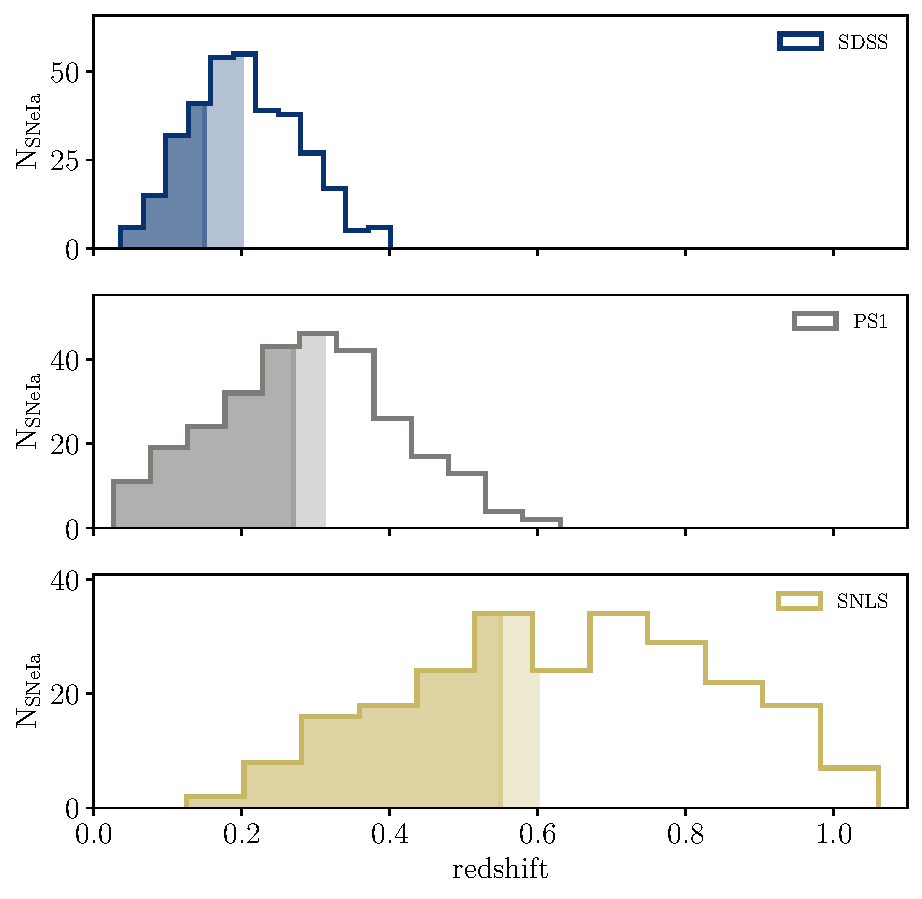
\includegraphics[width=0.80\linewidth]{hist_surveys_cuts}
    \caption[Histogrammes des sondages coupés pour notre étude]{\textit{De haut
        en bas}: Histogrammes en redshift des SNe~Ia des sondages SDSS, PS1 et
        SNLS~\citep[données de Pantheon,][]{scolnic2018}. Les parties colorées
        représentent les distribution de SNe~Ia conservées dans notre analyse,
        considérées exemptes d'effets de sélection observationnels (cf.
        Section~\ref{sssec:maglim}). Les couleurs foncées (claires) représentent
        les limites conservatives (fiducielles) nos coupes de sélection
    indiquées dans la Table~\ref{tab:zlimsample}.}
    \label{fig:cuts}
\end{figure}

En combinant les 5 sondages de notre analyse, on peut tracer leur distribution
de stretch en fonction du redshift. On en présente un graphique ainsi que
l'histogramme complet Figure~\ref{fig:sample}. En supposant l'échantillon
affranchi d'effets de sélection, on peut lire sur ce graphique une première idée
de l'évolution en redshift que l'on suppose issue du changement des propriétés
moyennes des SNe~Ia avec l'âge de leur environnement. En effet, on observe que
la fraction de SNe~Ia présentant un faible stretch, typiquement $x_1 < -1$,
semble décroître avec le redshift alors que la population de stretch $> 1$
semble toujours peuplée~; à noter qu'ici le redshift est en échelle
logarithmique, expliquant le tassement horizontal. Quantitativement, les SNe~Ia
à haut redshift présentent un plus grand stretch moyen ($0,34 \pm 0,10$ à
$z \approx 0,65$) que celles à bas redshift ($-0,17 \pm 0,10$ à $z \approx
0,05$). Cette idée est confirmée dans le chapitre suivant,
Section~\ref{sec:xres}.

\begin{figure}
    \centering
    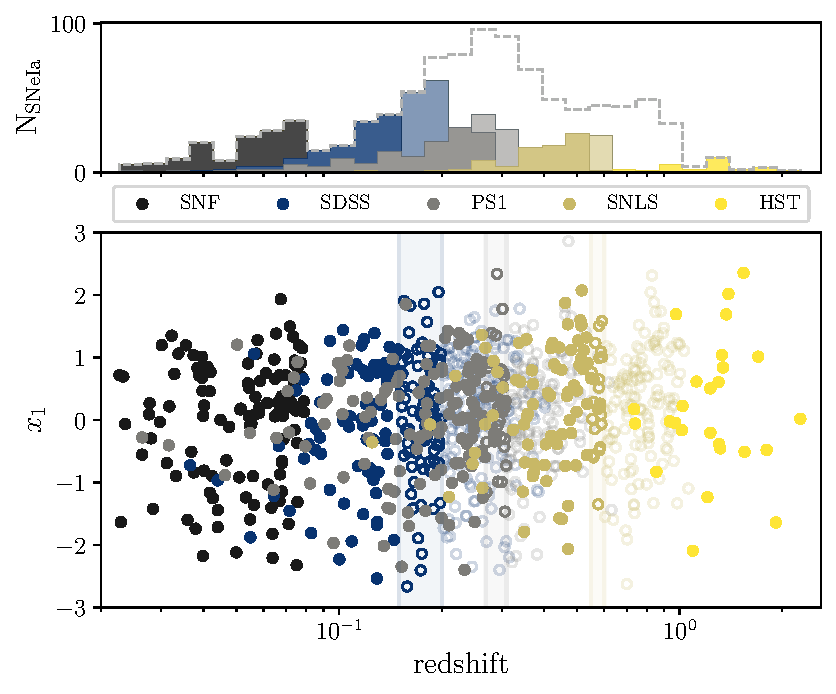
\includegraphics[width=0.95\linewidth]{stretchs-cut_btw_hist_stac.pdf}
    \caption[Présentation des données de stretch en fonction du
    redshift.]{\textit{En bas}~: stretch des courbes de lumière ajustées avec
        \textsc{\texttt{SALT2.4}} en fonction du redshift en échelle
        logarithmique pour chaque sondage de cette analyse (cf.~légende). Les
        points pleins (creux) correspondent aux limites conservatives
        (fiducielles). \textit{En haut}~: histogrammes en redshift superposés,
        en sombre (clair) pour les limites conservatives
    (fiducielles).}\label{fig:sample}
\end{figure}

\subsection{Confirmation d'hypothèse}\label{ssec:testvl}

% Dans la Section précédente, nous avons construit des échantillons limités en
% volume à partir d'ensembles limités en magnitude par le biais de simples coupes
% en redshift. Cette approche simplifiée est statistiquement sous-optimale, mais
% devrait suffire pour éprouver notre hypothèse concernant la compatibilité de
% l'évolution du stretch avec le redshift avec le modèle de \cite{rigault2020}.
% Cependant, il reste possible qu'une fonction complexe d'effets de sélection
% observationnels liée aux efficacités de suivi spectroscopique en-deçà de nos
% limites (fiducielles voire conservatives) affecte notre échantillon, le rendant
% de fait pas totalement limité en volume~; ceci biaiserait alors notre conclusion
% quant à l'existence d'une évolution astrophysique de la population des SNe~Ia.
% 
% Pour tester l'existence de biais de sélection observationnels résiduels dans
% notre échantillon, nous avons comparé 

Dans la Section précédente, nous avons construit des échantillons limités en
volume à partir d'un ensemble d'échantillons limités en magnitude en utilisant
des coupures simples de redshift. Cette approche simplifiée est
statistiquement sous-optimale, mais devrait suffire pour tester notre question
clé, à savoir si l'évolution du stretch avec le redshift est compatible avec le
modèle de \cite{rigault2020}. Cependant, il reste possible qu'une fonction de
sélection observationnelle complexe liée aux efficacités de suivi
spectroscopique en-deçà de nos coupures fiducielles (voire conservatives) puisse
encore affecter notre échantillon, le rendant non entièrement limité en volume~;
cela fausserait alors notre conclusion sur la dérive astrophysique de la
population SNe Ia.

Pour tester l'existence d'éventuels biais de sélection observationnels dans
notre échantillon, nous avons comparé les distributions de stretch et de couleur
des SNe~Ia provenant de différents ensembles de données dont les plages de
redshifts se chevauchent~: ces distributions devraient être similaires si elles
reflètent la même population mère sous-jacente. Nous notons que la plage de
redshift doit être suffisamment étroite pour que toute dérive soit négligeable.

Les deux échantillons qui se chevauchent le plus en termes de redshift sont PS1
et SDSS dans la plage de redshift $0,10 < z < 0,20$ (voir
Figure~\ref{fig:sample}). Ce sous-échantillon est constitué des 146 SNe~Ia à
l'extrémité haute des redshifts de SDSS et est donc le plus susceptible d'être
affecté par des effets de sélection observationnels résiduels (voir la
discussion correspondante dans la Section~\ref{ssec:malm}). Sur cette même plage
de redshift, PS1 compte 52 SNe~Ia qui se trouvent dans les tranches de redshift
les plus basses et qui sont donc peu susceptibles d'être affectées par un
problème de sélection observationnelle. Afin d'identifier les incohérences
potentielles entre les sous-échantillons PS1 et SDSS, la Figure~\ref{fig:testvl}
(panneaux supérieurs) compare la distribution des stretchs et des couleurs de
ces deux études. Les valeurs $p$ du test de similarité de
\textsc{Kolmogorov-Smirnov} (KS) qui en résultent ($p > 10\%$) n'indiquent
aucune incohérence, en accord avec l'impression visuelle de la
Figure~\ref{fig:testvl}.

\begin{figure}[ht]
    \centering
    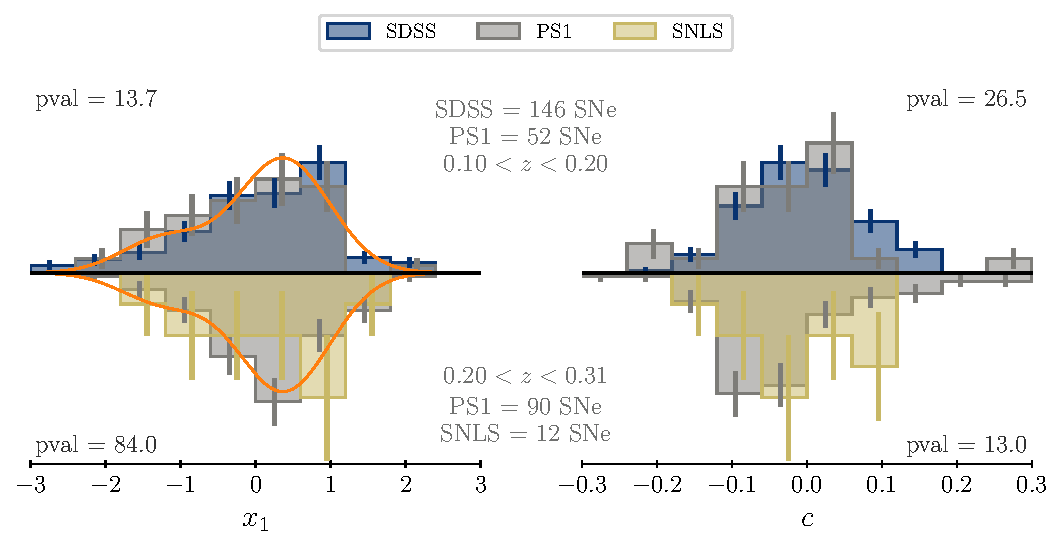
\includegraphics[width=.8\linewidth]{both-cut_SDSS_SNLS_PS1.pdf}
    \captionsetup{justification=centering}
    \caption{Histogrammes de distribution de stretch (gauche) et de couleur
        (droite) de différents relevés se chevauchant en redshift. \textit{Vers
        le haut}~: SDSS et PS1 dans la plage de redshift $0,10 < z < 0,20$.
        \textit{Vers le bas}~: PS1 et SNLS dans la gamme de redshift $0,20 < z <
        0,31$. Les barres d'erreur représentent le bruit de Poisson. Notre
        modèle d'évolution en redshift (défini plus loin,
        Section~\ref{ch:stretch}) est illustré en orange à la valeur moyenne des
        plages de redshifts, 0,15 et 0,25 respectivement. Les valeurs $p$ du
        test de \textsc{Kolmogorov-Smirnov} sont indiquées en haut (en bas) de
        chaque panneau et ne montrent aucun signe que les distributions de
        stretch et de couleur de SDSS et PS1 (PS1 et SNLS) ne sont pas tirées
    des mêmes distributions sous-jacentes.}
    \label{fig:testvl}
\end{figure}

Nous avons effectué une analyse similaire pour PS1 et SNLS sur la plage de
redshift $0,20 < z < 0,31$ (Figure~\ref{fig:testvl}, panneaux inférieurs), où la
même conclusion peut être tirée~: il n'y a pas de signe significatif de
divergence dans les distributions de stretch et de couleur entre les extrémités
basse et haute de nos échantillons fiduciels de SNLS et PS1, respectivement.
Néanmoins, la petite taille de l'ensemble de données SNLS à $z < 0,31$ (12
SNe~Ia contre 90 pour PS1) limite la sensibilité de ce test, et seule une forte
déviation serait perceptible. L'extension de la plage de redshift à $0,20 < z <
0,40$ (bien que nous n'ayons pas de données PS1 au-dessus de 0,3) permet
d'augmenter le sous-échantillon SNLS à 31, mais la valeur $p$ du stretch reste
élevée (34\%), ne montrant aucun signe d'incohérence.

Nous soulignons enfin que la couleur des SNe~Ia est plus sujette aux effets de
sélection observationnelle que le stretch, comme l'illustre la
Figure~\ref{fig:maglim}~; voir également la Figure~3 de~\cite{kessler2017}, par
exemple. Par conséquent, comme la comparaison des distributions de couleurs ne
montre aucune indication significative d'un effet de sélection observationnelle
résiduel, cela renforce notre affirmation selon laquelle nos critères de
sélection simples basés sur le redshift sont suffisants pour construire les
échantillons complets de SNe~Ia nécessaires pour tester l'évolution du redshift
de la distribution de stretch.

\newpage

% \dominilof
% \listoffigures
% \dominilot
% \listoftables
\minilof
\minilot

\bibliographystyle{../main/aa_url}
\shorthandoff{:}
\bibliography{../chapters/99_references}

\end{document}
